\pdfoutput=1
% Options for packages loaded elsewhere
\PassOptionsToPackage{unicode}{hyperref}
\PassOptionsToPackage{hyphens}{url}
\PassOptionsToPackage{dvipsnames,svgnames,x11names}{xcolor}
%
\documentclass[
  10pt,
]{article}
\usepackage{amsmath,amssymb}
\usepackage{iftex}
\ifPDFTeX
  % T1 fontenc omitted: OT1 Computer Modern (Type 1)
  \usepackage[utf8]{inputenc}
  \usepackage{textcomp} % provide euro and other symbols
\else % if luatex or xetex
  \usepackage{unicode-math} % this also loads fontspec
  \defaultfontfeatures{Scale=MatchLowercase}
  \defaultfontfeatures[\rmfamily]{Ligatures=TeX,Scale=1}
\fi
% lmodern omitted
\ifPDFTeX\else
  % xetex/luatex font selection
\fi
% Use upquote if available, for straight quotes in verbatim environments
\IfFileExists{upquote.sty}{\usepackage{upquote}}{}
\IfFileExists{microtype.sty}{% use microtype if available
  % microtype omitted
  % % disable protrusion for tt fonts
}{}
\makeatletter
\@ifundefined{KOMAClassName}{% if non-KOMA class
  \IfFileExists{parskip.sty}{%
    \usepackage{parskip}
  }{% else
    \setlength{\parindent}{0pt}
    \setlength{\parskip}{6pt plus 2pt minus 1pt}}
}{% if KOMA class
  \KOMAoptions{parskip=half}}
\makeatother
\usepackage{xcolor}
\usepackage[margin=2.2cm]{geometry}
\usepackage{longtable,booktabs,array}
\usepackage{calc} % for calculating minipage widths
% Correct order of tables after \paragraph or \subparagraph
\usepackage{etoolbox}
\makeatletter
\patchcmd\longtable{\par}{\if@noskipsec\mbox{}\fi\par}{}{}
\makeatother
% Allow footnotes in longtable head/foot
\IfFileExists{footnotehyper.sty}{\usepackage{footnotehyper}}{\usepackage{footnote}}
\makesavenoteenv{longtable}
\usepackage{graphicx}
\makeatletter
\def\maxwidth{\ifdim\Gin@nat@width>\linewidth\linewidth\else\Gin@nat@width\fi}
\def\maxheight{\ifdim\Gin@nat@height>\textheight\textheight\else\Gin@nat@height\fi}
\makeatother
% Scale images if necessary, so that they will not overflow the page
% margins by default, and it is still possible to overwrite the defaults
% using explicit options in \includegraphics[width, height, ...]{}
\setkeys{Gin}{width=\maxwidth,height=\maxheight,keepaspectratio}
% Set default figure placement to htbp
\makeatletter
\def\fps@figure{htbp}
\makeatother
\setlength{\emergencystretch}{3em} % prevent overfull lines
\providecommand{\tightlist}{%
  \setlength{\itemsep}{0pt}\setlength{\parskip}{0pt}}
\setcounter{secnumdepth}{-\maxdimen} % remove section numbering
\ifLuaTeX
\usepackage[bidi=basic]{babel}
\else
\usepackage[bidi=default]{babel}
\fi
\babelprovide[main,import]{english}
% get rid of language-specific shorthands (see #6817):
\let\LanguageShortHands\languageshorthands
\def\languageshorthands#1{}
\usepackage{caption}
\captionsetup{labelformat=empty,font=small}
\usepackage{float}
\floatplacement{figure}{!htbp}
\usepackage{needspace}
\usepackage{etoolbox}
\pretocmd{\section}{\Needspace{10\baselineskip}}{}{}
\pretocmd{\subsection}{\Needspace{7\baselineskip}}{}{}
\usepackage{lastpage}
\usepackage{fancyhdr}
\fancypagestyle{plain}{\fancyhf{}\renewcommand{\headrulewidth}{0pt}\fancyfoot[C]{\small\thepage\,/\,\pageref*{LastPage}}}
\pagestyle{plain}
\widowpenalty=10000
\clubpenalty=10000
\DeclareUnicodeCharacter{2212}{\ensuremath{-}}
\DeclareUnicodeCharacter{00B1}{\ensuremath{\pm}}
\DeclareUnicodeCharacter{00D7}{\ensuremath{\times}}
\DeclareUnicodeCharacter{2192}{\ensuremath{\rightarrow}}
\DeclareUnicodeCharacter{222A}{\ensuremath{\cup}}
\DeclareUnicodeCharacter{2264}{\ensuremath{\le}}
\DeclareUnicodeCharacter{2026}{\ldots}
\DeclareUnicodeCharacter{201C}{\textquotedblleft}
\DeclareUnicodeCharacter{201D}{\textquotedblright}
\ifLuaTeX
  \usepackage{selnolig}  % disable illegal ligatures
\fi
\IfFileExists{bookmark.sty}{\usepackage{bookmark}}{\usepackage{hyperref}}
\IfFileExists{xurl.sty}{\usepackage{xurl}}{} % add URL line breaks if available
\urlstyle{same}
\hypersetup{
  pdftitle={Different instruments, the same chord: the comb of
resonances and the first-order phase for Dirichlet L-functions with
complex characters, the cyclotomic union, and the robustness of the main
resonance of study VI - a reproducible numerical study VII},
  pdfauthor={David Hess (MAYAN ALFA V1008 LAB v.34.116)},
  pdflang={en},
  colorlinks=true,
  linkcolor={Maroon},
  filecolor={Maroon},
  citecolor={Blue},
  urlcolor={Blue},
  pdfcreator={LaTeX via pandoc}}

\title{Different instruments, the same chord: the comb of resonances and
the first-order phase for Dirichlet L-functions with complex characters,
the cyclotomic union, and the robustness of the main resonance of study
VI --- a reproducible numerical study VII}
\author{David Hess (MAYAN ALFA V1008 LAB v.34.116)}
\date{23 November 2026}

\begin{document}
\maketitle
\begin{abstract}
Study VI of this series measured a comb of resonances in the variance of
the windowed sums \(\sum g\,x^{i\gamma}\) over the zeros of \(\zeta\)
and of Dirichlet L-functions with real characters, in agreement with the
two-point functions of Bogomolny and Keating. Here the measurement is
extended to complex characters, and the question is what depends on the
character and what only on its modulus. Every rule was recorded before
the zeros were computed or, for the later additions, before the quantity
was evaluated. On 1,296,658 newly computed zeros of 16 Dirichlet
L-functions modulo 5, 7, 13, 15 and 21 between heights 36,000 and 80,000
(twelve with complex characters and four that complete the families
modulo 15 and 21): (1) for the twelve L-functions with complex
characters the comb depends on the modulus only --- mean \(z^2\) over
201 points 0.13--0.25 against the two-point function with the Euler
factors of \(p \mid q\) removed and 11.5--49 against GUE without
arithmetic, with the same comb for all 18 pairs of L-functions of one
modulus; (2) the first order carries the phase of \(\chi(p)\): the first
Fourier coefficient of \(\{\gamma\ln p/2\pi\}\) equals
\(-w\chi(p)\ln p/\sqrt p\) to \(5.2\cdot10^{-5}\) in 56 combinations of
these L-functions and primes, and the conjugate phase is excluded; (3)
in the union of all characters of a modulus, which is the set of zeros
of the Dedekind zeta function of \(\mathbb{Q}(\zeta_q)\) for
\(q = 5, 7, 15, 21\) (up to 947,573 zeros), a prime sounds only in the
harmonics that are multiples of its order modulo \(q\); (4) L-functions
of one modulus share their primes, and the cross-covariance of their
windowed sums equals the prime trace with the relative phase
\(\chi_a\bar\chi_b\); (5) the number variance saturates at a level set
by the modulus; (6) the main resonance of study VI holds for another
window, six error estimates and the full covariance of the scan, with
GUE between 12 and 69 errors away depending on the error estimate.

Three blind tests turn this into a use: from the zeros alone the modulus
and the character, the primes dividing the modulus, and the orders of 16
primes in four cyclotomic fields were identified correctly, 16 of 16 in
each test. Three further measurements connect the data with random
matrices: the pair correlation of each L-function up to three mean
spacings follows the two-point function of Bogomolny and Keating
(\(\chi^2\) per bin 0.78--1.86) and not GUE alone (6.3--16.5); the
spacings of the unions agree with a superposition of independent GUE
spectra, one for each character, to 0.010 in the density, with a small
deficit of the smallest spacings; and the deviation from GUE fades with
height as predicted: between the bands 36,000--80,000 and
400,000--420,000 its size falls to \(0.719 \pm 0.021\) of its value,
against 0.727 predicted. A count test of Turing type found two pairs of
close zeros that the search grid had stepped over; they were repaired
before the evaluation. The one wrong reading outside the tests, the
order of 11 in \(\mathbb{Q}(\zeta_{21})\), is explained by the
resolution of the band: near \(11^5\) the union hears the prime 161,071
twenty steps away. All 18 hypotheses are supported. The statements
tested in (2)--(4) are theorems or direct consequences of them; the
two-point function behind (1), (5), (6) and the pair correlation is a
conjecture. What is added is data for complex characters with null
models and errors, zeros that did not exist when the rules were written,
and the blind tests.
\end{abstract}

\hypertarget{introduction}{%
\section{1. Introduction}\label{introduction}}

Study VI of this series {[}6{]} measured the variance of the windowed
sum \(\sum_\gamma g\,x^{i\gamma}\) over the zeros of \(\zeta\) and found
a comb of resonances at \(x = (T/2\pi)\cdot A/B\), in agreement with the
two-point function of Bogomolny and Keating {[}7{]} and far from random
matrices without arithmetic. For eight Dirichlet L-functions with real
characters \(\chi_D\) the comb agreed with the two-point function for
Dirichlet L-functions {[}8{]}, which differs from that of \(\zeta\) only
by finite products over the primes dividing the modulus. Two questions
were left open: whether the same holds for complex characters, and how
robust the main resonance is against choices of the measurement (window
shape, error estimate, correlated points).

For a single L-function \(L(s, \chi)\) in the \(t\)-aspect, the
arithmetic factor of the two-point function contains \(|\chi(n)|^2\), so
its prediction depends on the modulus \(q\) and not on the values of
\(\chi\) {[}8{]}. The first-order effect is different: by Landau's
formula for \(L(s, \chi)\) {[}9, 10{]},
\[\sum_{T_1 < \gamma \le T_2} x^{\rho} = -\frac{T_2 - T_1}{2\pi}\,\chi(x)\Lambda(x) + O(\ln T_2),\]
so the first Fourier coefficient of the fractional parts
\(\{\gamma\ln p/2\pi\}\) carries the phase of \(\chi(p)\), and the dip
of their density moves from \(0\) to \(\arg\chi(p)/2\pi\). In the
language of a hypothetical spectral interpretation (Hilbert--Pólya;
Berry and Keating {[}11{]}) the primes play the role of periodic orbits
of length \(\ln p\), the explicit formula is a trace formula, and a
character acts like a phase attached to each orbit. A phase of this kind
is seen by single orbits (first order) and cancels in the pairing of an
orbit with itself (second order). The present study measures both sides
of this statement on new zeros.

Four further comparisons use data that already exist. The zeros of all
characters modulo \(q\) together are the zeros of the Dedekind zeta
function of the cyclotomic field \(\mathbb{Q}(\zeta_q)\); in this union
the first-order terms cancel except at prime powers
\(p^k \equiv 1 \pmod q\), so the zeros should reflect how primes split
in the field. This is the number-theoretic analogue of the decomposition
of a spectrum with a discrete symmetry into symmetry sectors {[}12,
13{]}. Second, different L-functions of the same modulus share the
primes, so the windowed sums of two such L-functions are correlated,
with the relative phase \(\chi_a(p)\overline{\chi_b(p)}\), wherever few
primes contribute. Third, the number variance of the zeros saturates at
a level set by the primes (Berry {[}14{]}); for \(L(s, \chi)\) it should
again depend on \(q\) only. Fourth, the first zeros of all twelve
L-functions are compared with the LMFDB {[}15{]}.

Two further parts were added by dated addenda before the data they
concern were evaluated. Three blind tests ask whether the comb and the
first order are enough to recognise, from zeros alone, an L-function,
the primes dividing its modulus and the splitting of primes in a
cyclotomic field (Section 5). Three measurements connect the data with
random-matrix theory: the pair correlation of a single L-function at
short range, the spacings of the unions against a superposition of
independent spectra, and the dependence of the deviation from GUE on the
height (Section 3.9).

The study is numerical. Every formula tested is either a theorem or a
direct consequence of one (Landau's formula, the explicit formula,
orthogonality of characters) or a conjecture with an explicit prediction
(the two-point function of Bogomolny and Keating). Nothing here bears on
the Riemann hypothesis or on the existence of a Hamiltonian; the
measurements are conditions that any such construction would have to
meet.

\hypertarget{data}{%
\section{2. Data}\label{data}}

\textbf{Twelve new L-functions (set hr7).} Primitive characters modulo
\(q = 5\) (order 4), \(7\) (orders 3 and 6), \(13\) (order 12), \(15\)
(order 4, \(p \mid q\): 3, 5) and \(21\) (order 6, \(p \mid q\): 3, 7),
each with its complex conjugate --- Conrey labels 5.2, 5.3; 7.2, 7.4,
7.3, 7.5; 13.2, 13.7; 15.2, 15.8; 21.5, 21.17. All zeros with
\(36{,}000 < \gamma \le T_2\) were computed with PARI/GP 2.17.2 {[}16{]}
(\texttt{lfunzeros}, windows of width 100, \texttt{divz} 32,
completeness checked against the smooth count
\((\theta_\chi(b) - \theta_\chi(a))/\pi\) in every window) on a desktop
computer (9 processes) after the rules of this study had been recorded;
\(T_2 = 80{,}000\) was reached for all twelve (counts and times in
Section 4.1).

\textbf{Four further L-functions (set hr7b).} To complete the families
of all characters modulo 15 and modulo 21, the zeros of
\(L(s, \chi_{-15})\) (15.14), \(L(s, \chi_{21})\) (21.20) and of the
second complex pair of order 6 modulo 21 (21.2, 21.11) were computed in
the same band with the same script after the main run (addendum 5 to the
rules): 82,726, 85,082, 85,083 and 85,082 zeros after the repair of
Section 4.10. With \(\zeta\), \(\chi_{-3}\), \(\chi_5\), \(\chi_{-7}\)
of study VI and set hr7 this gives all 8 characters modulo 15 and all 12
modulo 21, each imprimitive character being represented by the primitive
character that induces it. Sets hr7 and hr7b together are the 16
L-functions of this study, with 1,296,658 zeros.

\textbf{A second band (set hr7c).} For the comparison of two heights
(Section 3.9) the zeros of the four L-functions of set hr7b with
\(400{,}000 < \gamma \le 420{,}000\) were computed with the same script
on 22 November 2026, after the rules of that comparison and its
evaluation script had been recorded: 178,844 zeros, computed on the same
desktop computer from 20:03 to 23:32 UTC (first and last window).

\textbf{Reference data from earlier studies.} The zeros of
\(L(s, \chi_5)\), \(L(s, \chi_{-7})\), \(L(s, \chi_{13})\) in the same
band (study VI {[}6{]}); the zeros of \(\zeta\) in the same band from
the tables of Platt {[}17{]} in the LMFDB {[}15{]} (agreement with
Odlyzko's zeros6 {[}18{]} to \(3\cdot10^{-9}\)); and for the robustness
part the two bands of Platt's zeros at \(t \approx 10^8\) (P8) and
\(t \approx 3\cdot10^{10}\) (P3e10) used in study VI.

\textbf{Checks.} Forty random zeros of each L-function evaluated in
mpmath through the Hurwitz zeta function; the first 25 zeros of each of
the twelve L-functions compared with the LMFDB (largest difference
\(3.6\cdot10^{-15}\)); the zeros of \(L(s, \chi)\) below the real axis
coincide with those of \(L(s, \bar\chi)\) above it.

\hypertarget{methods}{%
\section{3. Methods}\label{methods}}

\hypertarget{the-comb-of-a-single-l-function}{%
\subsection{3.1 The comb of a single
L-function}\label{the-comb-of-a-single-l-function}}

As in study VI {[}6{]}: Gaussian windows of width \(H = 20\) with
centres \(T_0\) spaced by \(H\), \(\ln x = \ln(qT_0/2\pi) + \delta\)
with \(\delta \in [-2.5, 2.5]\) in steps of 0.025,
\(V(\delta) = \langle|S - \langle S\rangle|^2\rangle/\langle N_2\rangle\),
error = the larger of \(V/\sqrt M\) (\(M\) independent windows spaced by
\(6H\)) and the scatter over ten sub-bands. Prediction
\(V_{\mathrm{BK},q}\): the two-point function of \(\zeta\) with the
Euler factors of \(p \mid q\) removed and \(L = \ln(qT/2\pi)\) {[}8{]},
computed by the code of study VI unchanged (identical to the published
predictions for \(q = 5, 7, 13\)). Null predictions: the same function
without removing the factors (``naive \(\zeta\)'') and GUE without
arithmetic.

\hypertarget{same-modulus-same-comb-without-theory}{%
\subsection{3.2 Same modulus, same comb (without
theory)}\label{same-modulus-same-comb-without-theory}}

For two L-functions \(a\), \(b\) of the same modulus,
\(Q_{ab} = \langle (V_a - V_b)^2/(e_a^2 + e_b^2)\rangle_\delta\).
Control pairs of different moduli, where the theory predicts a
difference (\(Q_{ab} \approx 15\)--20), show that the test can see one.

\hypertarget{the-first-order-phase}{%
\subsection{3.3 The first-order phase}\label{the-first-order-phase}}

For each L-function and prime \(p \nmid q\), \(p \le 13\):
\(c = \langle e^{2\pi i u}\rangle\) with \(u = \{\gamma\ln p/2\pi\}\),
prediction \(c = -w\,\chi(p)\ln p/\sqrt p\), \(w = (T_2 - T_1)/2\pi N\);
histogram of \(u\) against the density
\(1 - 2w\sum_k (\ln p/p^{k/2})\,\mathrm{Re}(\chi(p)^k e^{-2\pi i k u})\)
and against the conjugate phase.

\hypertarget{the-cyclotomic-union}{%
\subsection{3.4 The cyclotomic union}\label{the-cyclotomic-union}}

\(U_5 = \{\zeta, \chi_5, \chi, \bar\chi\}\) and
\(U_7 = \{\zeta, \chi_{-7}\), two pairs of order 3 and 6\(\}\):
\(c_k(p) = -w_U\,\varphi(q)\,[p^k \equiv 1 \bmod q]\,\ln p/p^{k/2}\) for
\(x = p^k \le 200\); histograms for \(p = 2, 3\) against the
interference prediction and against an alternative without interference.

\hypertarget{shared-orbits-cross-covariance}{%
\subsection{3.5 Shared orbits:
cross-covariance}\label{shared-orbits-cross-covariance}}

\(C_{ab}(x) = \langle (S_a - \langle S_a\rangle)\overline{(S_b - \langle S_b\rangle)}\rangle/\sqrt{N_{2,a}N_{2,b}}\)
at \(\ln x \in \{3,\penalty300 4,\penalty300 5,\penalty300 6\}\) against the prime trace
\((H^2/2\pi)\sum_n \chi_a(n)\overline{\chi_b(n)}\Lambda(n)^2 n^{-1}e^{-H^2\ln^2(n/x)}/\sqrt{N_{2,a}N_{2,b}}\).

\hypertarget{saturation-of-the-number-variance}{%
\subsection{3.6 Saturation of the number
variance}\label{saturation-of-the-number-variance}}

\(\Sigma^2(\ell)\) of the unfolded zeros (\(\theta_\chi(\gamma)/\pi\)),
intervals starting every 0.37, \(\ell \in [0.1, 200]\), error from ten
sub-bands; prediction from the two-point function of Bogomolny and
Keating without the factors \(p \mid q\) (validated against the code of
study VI to \(5\cdot10^{-5}\)); Berry's diagonal formula {[}14{]} for
comparison.

\hypertarget{robustness-of-the-main-resonance-zeros-of-zeta}{%
\subsection{\texorpdfstring{3.7 Robustness of the main resonance (zeros
of
\(\zeta\))}{3.7 Robustness of the main resonance (zeros of \textbackslash zeta)}}\label{robustness-of-the-main-resonance-zeros-of-zeta}}

Hann window \(\cos^2(\pi t/2a)\), \(a = 3H\), with the prediction
recomputed for its autocorrelation (checked against a sieve in the
diagonal regime to \(8\cdot10^{-7}\)); six error estimates at
\(\tau = 1\) (5, 10, 20, 40 sub-bands, \(V/\sqrt M\), block jackknife);
the full covariance of the 201-point scan with Hotelling's correction,
the effective number of independent points and a global \(p\)-value for
the largest deviation. The same Hann analysis for the twelve
L-functions.

\hypertarget{rules-recorded-beforehand}{%
\subsection{3.8 Rules recorded
beforehand}\label{rules-recorded-beforehand}}

The rules of this study were written on 20 November 2026 at 07:58 UTC,
before the zeros of set hr7 were computed (the first window was written
at 08:03 UTC). Three dated addenda followed, all before the data were
transferred from the desktop computer: the fingerprints of the
evaluation scripts after a rehearsal on a test L-function (09:15 UTC),
five additional comparisons proposed with the data still unseen (15:14
UTC), and two corrections found on test data --- the number variance is
compared with the full two-point function rather than Berry's diagonal
formula, and the cyclotomic union is judged only for \(x \le 200\),
where the error term of Landau's formula is small (15:51 UTC). What had
been computed from the band before the rules (timing runs only, no
statistics) is listed in them.

\hypertarget{random-matrix-comparisons-addenda-9-and-10}{%
\subsection{3.9 Random-matrix comparisons (addenda 9 and
10)}\label{random-matrix-comparisons-addenda-9-and-10}}

The zeros of a single L-function high on the critical line are
conjectured to follow, locally, the statistics of the eigenvalues of
large random unitary matrices (GUE): Montgomery {[}22{]} for the pair
correlation of \(\zeta\), the numerical evidence of Odlyzko {[}23{]},
and Rudnick and Sarnak {[}24{]} for principal L-functions in restricted
ranges. At finite height there are arithmetic corrections. For \(\zeta\)
they follow from the two-point function of Bogomolny and Keating {[}7{]}
and were compared with data by Bogomolny, Bohigas, Leboeuf and Monastra
{[}25{]}, who showed that to leading order the zeros near height \(T\)
behave like eigenvalues of unitary matrices of a finite effective size.
For Dirichlet L-functions the two-point function of {[}8{]} contains the
same kind of correction with the Euler factors of the primes dividing
\(q\) removed; {[}8{]} gives no numerical comparison. Three measurements
connect the present data with this picture. Their rules were recorded on
22 November 2026, after the fifteen tests above had been evaluated but
before any of these statistics was computed.

\begin{enumerate}
\def\labelenumi{(\roman{enumi})}
\item
  \emph{Pair correlation at short range.} With the unfolding
  \(w = (\gamma/2\pi)(\ln(q\gamma/2\pi) - 1)\), the density \(R_2(d)\)
  of pairs at unfolded distance \(0 < d \le 3\) is measured in 60 bins
  of width 0.05, with errors from ten blocks, and compared with the GUE
  form \(1 - (\sin\pi d/\pi d)^2\) and with the two-point function of
  {[}8{]}, averaged over each bin and over the band. Pass mark:
  \(\chi^2\) per bin at most 2.0 against {[}8{]} for at least 14 of the
  16 L-functions, with GUE at least three times worse and at least 4.
\item
  \emph{The union as a superposition.} If the sectors of a union (the
  L-functions of the characters modulo \(q\)) were statistically
  independent GUE spectra with density fractions \(f_i\), the
  probability that an interval of \(s\) mean spacings of the union is
  empty would be \(E_S(s) = \prod_i E_\mathrm{GUE}(f_i s)\), and the
  spacing density \(p_S = E_S''\) --- the superposition rule of
  Rosenzweig and Porter {[}27{]} and of Berry and Robnik {[}28{]}. That
  the zeros of different L-functions are statistically independent, so
  that the zeros of a product behave like a superposition of
  uncorrelated GUE sets, was argued by Bogomolny and Leboeuf {[}30{]} on
  the assumption of the Hardy--Littlewood conjecture. \(E_\mathrm{GUE}\)
  is the Fredholm determinant of the sine kernel, evaluated by
  Gauss--Legendre quadrature {[}26{]}. Pass mark, for all four unions:
  largest \(|p - p_S|\) over 40 bins of width 0.1 at most 0.015; first
  bin at least 0.03 below the Poisson value; a single GUE spectrum off
  by at least 0.2 in some bin.
\item
  \emph{Height.} The pair correlation of (i) is measured again for the
  four L-functions of set hr7b in a second band,
  \(400{,}000 < \gamma \le 420{,}000\), whose zeros were computed after
  the rules were recorded. There {[}8{]} predicts a smaller deviation
  from GUE. The measured deviation is summarized by the amplitude \(A\)
  of \(R_2 - R_2^\mathrm{GUE}\) along the predicted shape
  \(R_2^\mathrm{BK} - R_2^\mathrm{GUE}\) (weighted by the block errors)
  and by its size
  \(V = A\cdot\mathrm{rms}(R_2^\mathrm{BK} - R_2^\mathrm{GUE})\), pooled
  over the four L-functions. Pass marks: \(\chi^2\) per bin at most 2.0
  in the upper band for at least three of the four; pooled \(|A - 1|\)
  within three errors; pooled size smaller in the upper band by at least
  three errors; ratio of the sizes within three errors of the predicted
  ratio.
\end{enumerate}

The symmetry type of a family in the sense of Katz and Sarnak {[}29{]}
--- unitary for all characters of a modulus, symplectic for the
quadratic characters of studies III and V --- concerns low-lying zeros
across a family. It is not tested here: all zeros of this study lie high
on the critical line.

\hypertarget{the-laboratory-and-the-use-of-an-ai-assistant}{%
\subsection{3.10 The laboratory and the use of an AI
assistant}\label{the-laboratory-and-the-use-of-an-ai-assistant}}

\textbf{Laboratory.} The measurements were developed in the laboratory
named in the author line (a development tool of the author; it is not
part of the publication). Every hypothesis is entered there with its
rule, its null model and its verdict, and the sheet of this study
recomputes the main quantities from stored counts and compares them with
the results of the scripts. The laboratory is a check of the
bookkeeping, not a source of numbers: every number of this article is in
the results files of the repository.

\textbf{Use of an AI assistant.} The work was done in a dialogue between
the author and an AI assistant (Claude, Anthropic). The author set the
questions and the scope, decided what would be measured and what the
rules would require, ran the computations of the zeros on his own
computer, and approved every step and this text. The assistant wrote and
ran the scripts, searched the literature, drafted the rules and drafted
the article in English and in Czech. No number in the article comes from
a language model: every number is computed by a script of the repository
(PARI/GP, mpmath, NumPy, SciPy, python-flint) from the data of Section 2
and is stored in the results files; the evaluation scripts were
fingerprinted (SHA-256) before the data they evaluate were opened, and
the main numbers are recomputed by independent code. Errors found on the
way --- among them the two missed pairs of zeros of Section 4.10 --- are
recorded in the dated addenda and not removed. The responsibility for
the content rests with the author.

\hypertarget{results}{%
\section{4. Results}\label{results}}

\hypertarget{data-1}{%
\subsection{4.1 Data}\label{data-1}}

The twelve L-functions have 75,032 to 85,082 zeros each in
\(36{,}000 < \gamma \le 80{,}000\), 958,685 in total; all 440 windows of
each L-function are present with matching SHA-256 fingerprints, the
zeros are increasing, and over the whole band the counts differ from the
smooth count by at most 1.1. Forty random zeros of each L-function give
\(|L(\tfrac12 + i\gamma, \chi)| \le 1.3\cdot10^{-9}\) in mpmath. The
computation ran on the desktop computer from 20 November 08:03 UTC to
23:13 UTC; nine windows interrupted by a keyboard interrupt in the
terminal were recomputed on the same computer with the same command on
21 November (00:41--00:43 UTC) and agree bit for bit with an independent
recomputation in the cloud. When the same command was started again, the
desktop computer also recomputed 4,397 of the 5,280 windows a second
time (21 November, 00:44--18:23 UTC); all of them are identical bit for
bit with the first computation.

\hypertarget{one-chord-for-every-instrument}{%
\subsection{4.2 One chord for every
instrument}\label{one-chord-for-every-instrument}}

For all twelve L-functions the comb agrees with the prediction
\(V_{\mathrm{BK},q}\): \(Q = 0.13\)--\(0.25\) on 201 points (2,183
windows, \(M = 364\)), largest \(|z| = 1.66\) (Fig. 1). GUE without
arithmetic gives \(Q = 11.5\)--\(49\) on the same errors, the naive
\(\zeta\) prediction (factors \(p \mid q\) not removed)
\(Q = 3.3\)--\(64\). For \(q = 13\) the naive prediction cannot be told
apart (\(Q = 0.78\)); the rules had stated in advance that the test has
little power there (expected \(Q = 0.6\)), because the first tooth
affected by \(p = 13\) lies outside the scanned range. The height of the
tooth at the ratio \(A/B = 2\) follows the modulus:

{\small\begin{longtable}[]{@{}llll@{}}
\toprule\noalign{}
\(q\) & primes removed & measured (each L-function) & predicted \\
\midrule\noalign{}
\endhead
\bottomrule\noalign{}
\endlastfoot
5 & 5 & 3.78, 3.87 (\(\pm 0.20\)) & 3.81 \\ \addlinespace[2pt]
7 & 7 & 3.30--3.33 (\(\pm 0.17\)) & 3.33 \\ \addlinespace[2pt]
13 & 13 & 2.90, 2.91 (\(\pm 0.15\)) & 2.87 \\ \addlinespace[2pt]
15 & 3, 5 & 7.15, 7.11 (\(\pm 0.37\)) & 7.15 \\ \addlinespace[2pt]
21 & 3, 7 & 6.23, 6.11 (\(\pm 0.33, \pm 0.32\)) & 6.16 \\ \addlinespace[2pt]
\end{longtable}}

Without any theory, the 18 pairs of L-functions of the same modulus
(including the real characters of study VI) have the same comb,
\(Q_{ab} = 0.13\)--\(0.29\), while control pairs of different moduli
differ, \(Q_{ab} = 15.3\)--\(20.1\).

The values \(Q \approx 0.15\) instead of \(\approx 1\) mean that the
error estimate of the comb is conservative by a factor of about 2.5. The
same was seen in study VI and on the test L-function \(q = 11\); it does
not reduce the separation from the null predictions, which are judged on
the same errors.

\begin{figure}
\centering
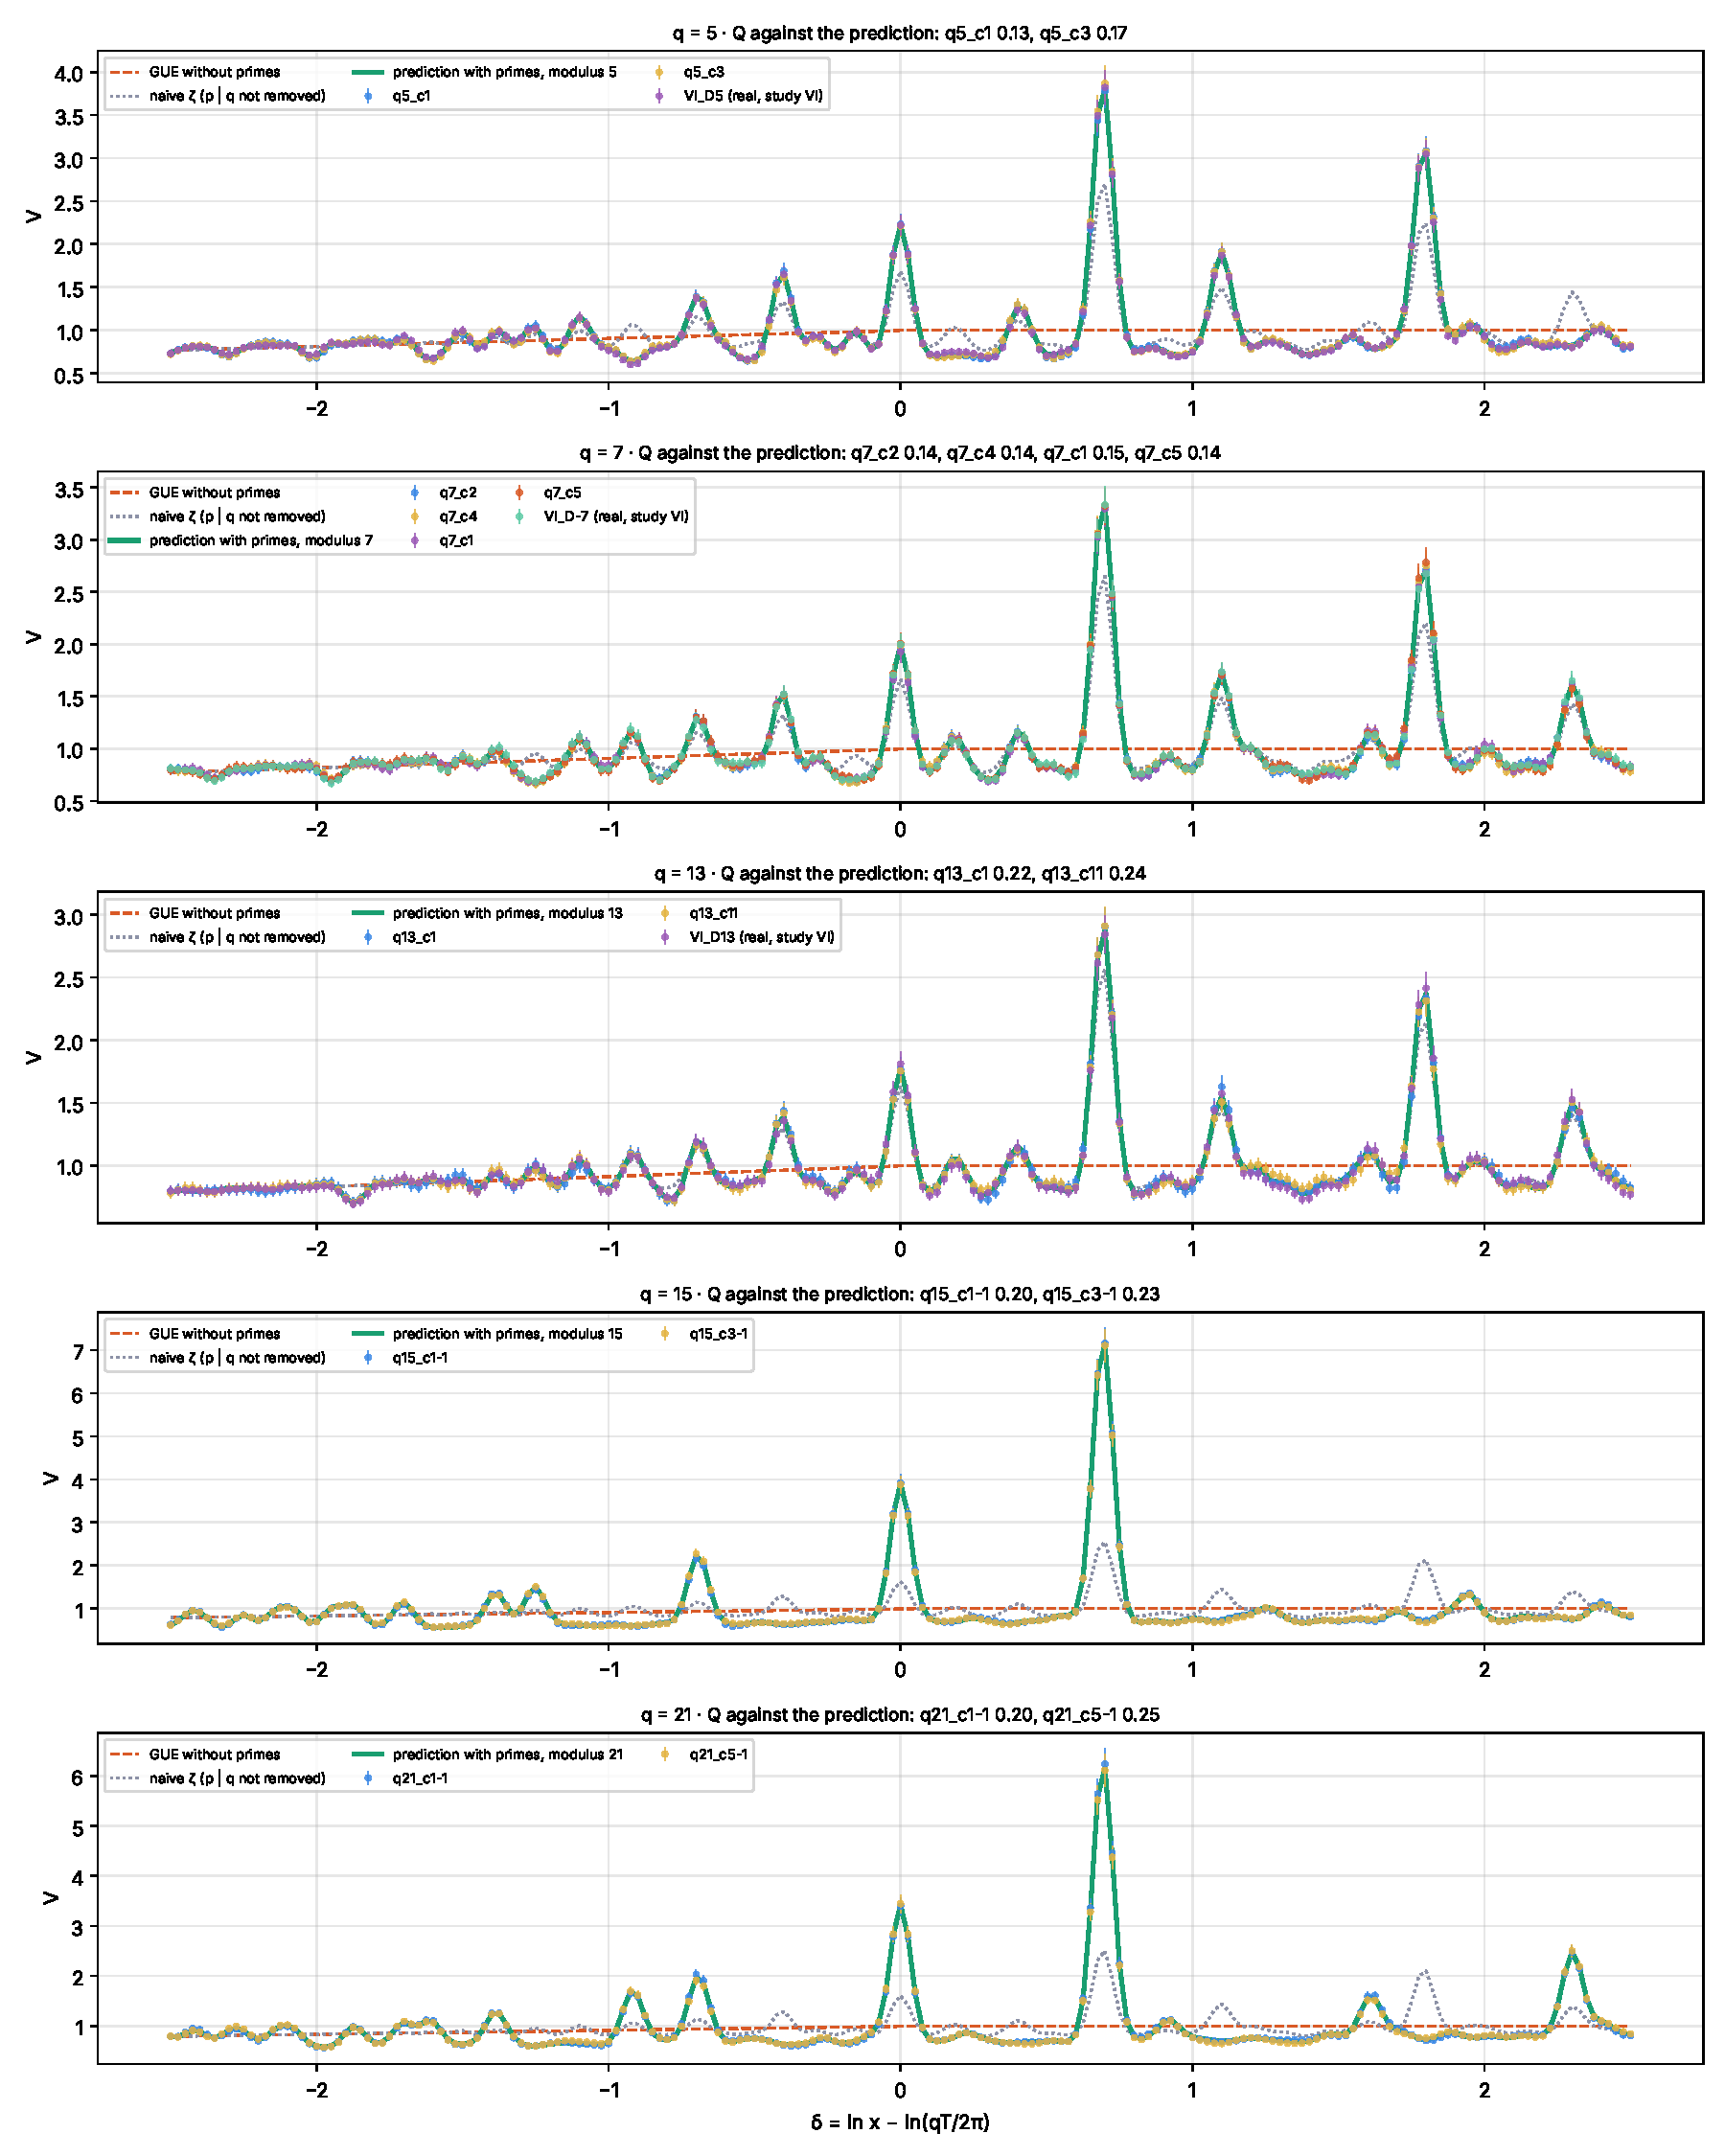
\includegraphics[width=1\textwidth,height=\textheight]{../figures/01_comb_en.pdf}
\caption{Figure 1. The comb of resonances by modulus: \(V(\delta)\) of
the twelve L-functions of set hr7 and of the real characters of study VI
(\(\pm 1\) error, heights 36,000--80,000, \(H = 20\), 201 points)
against the two-point function with the Euler factors of \(p \mid q\)
removed (solid), the naive \(\zeta\) prediction (dotted) and GUE without
arithmetic (dashed).}
\end{figure}

\hypertarget{the-melody-carries-the-phase}{%
\subsection{4.3 The melody carries the
phase}\label{the-melody-carries-the-phase}}

For the 56 combinations of an L-function and a prime \(p \le 13\),
\(p \nmid q\), the first Fourier coefficient of \(\{\gamma\ln p/2\pi\}\)
agrees with \(-w\,\chi(p)\ln p/\sqrt p\) to \(5.2\cdot10^{-5}\) (Fig.
2); the histograms agree with the density built from \(\chi(p)\)
(smallest \(p = 0.13\)), and for all 46 combinations with complex
\(\chi(p)\) the conjugate phase is rejected (\(p \le 7\cdot10^{-154}\)).
The dip of the density moves to \(\arg\chi(p)/2\pi\) as stated by
Landau's formula. The \(\chi^2\) values of the histograms are mostly
smaller than their number of degrees of freedom (\(p\) between 0.75 and
1): the fractional parts are more evenly spread than independent points
would be, a consequence of the rigidity of the zeros.

The windowed sums agree with the sieve over prime powers to
\(1.4\cdot10^{-11}\) (960 points, sharp window up to
\(6.2\cdot10^{-2}\)), and in the diagonal regime the data agree with the
prime sum to \(|z| \le 0.06\). An independent second implementation of
the comb and of the coefficients reproduces the first to
\(5.9\cdot10^{-12}\) and \(1.1\cdot10^{-12}\).

\begin{figure}
\centering
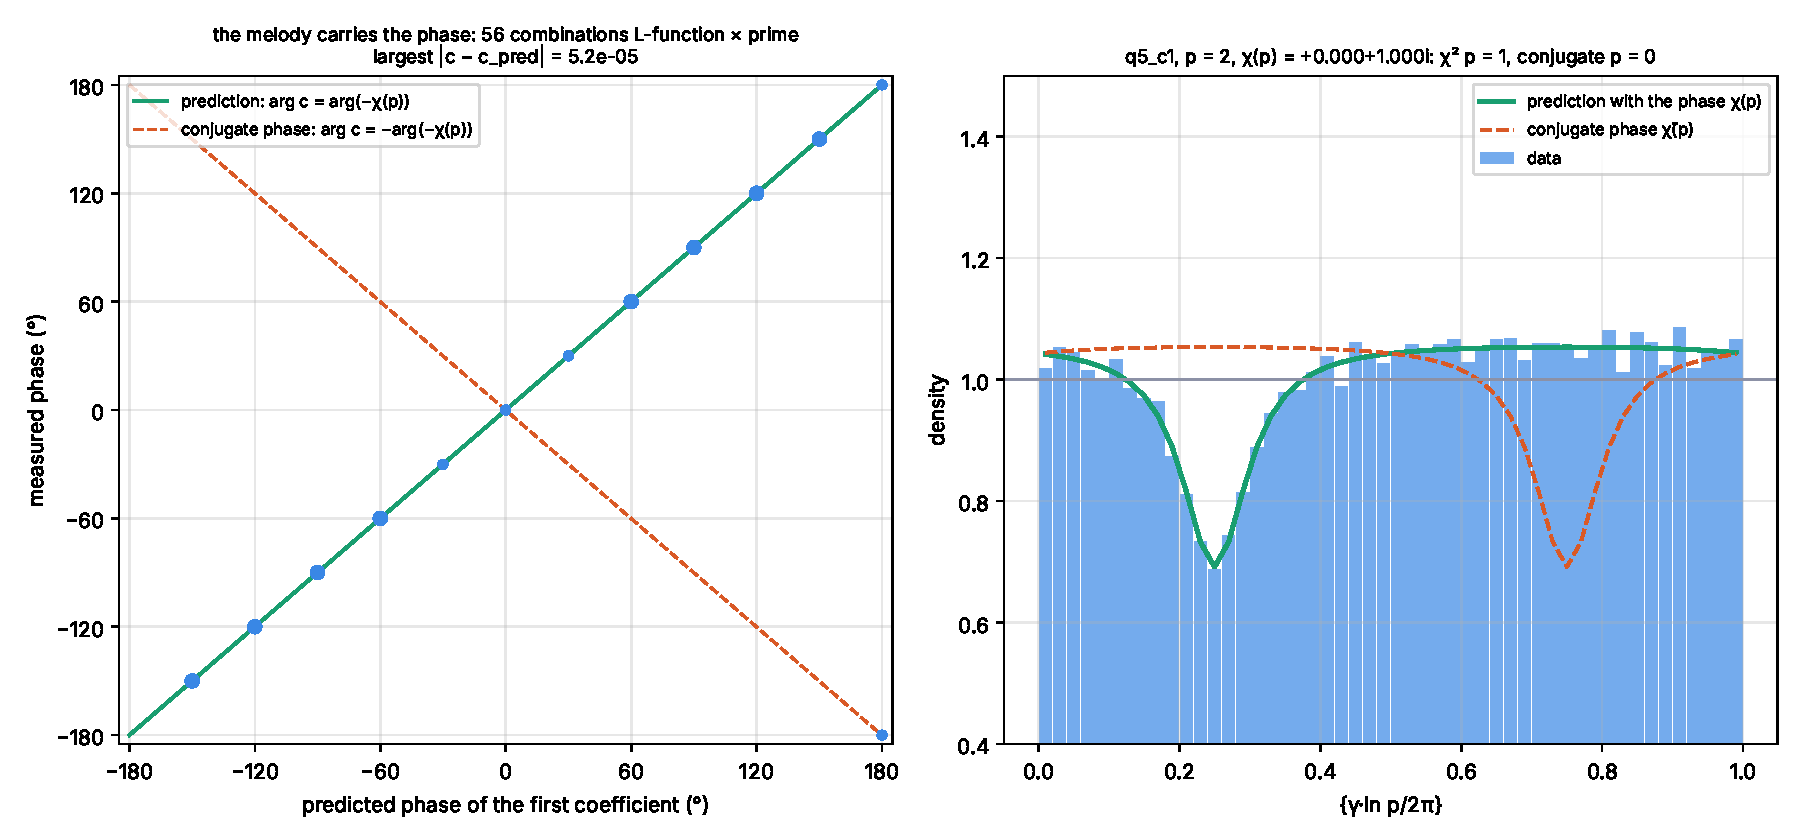
\includegraphics[width=1\textwidth,height=\textheight]{../figures/02_phase_en.pdf}
\caption{Figure 2. The first-order phase. Left: measured against
predicted phase of the first Fourier coefficient of
\(\{\gamma\ln p/2\pi\}\) for the 56 combinations of an L-function and a
prime; the conjugate phase would lie on the falling line. Right: an
example histogram (5.2, \(p = 2\), \(\chi(2) = i\)) with the density
built from \(\chi(p)\) and from its conjugate.}
\end{figure}

\hypertarget{the-whole-orchestra-the-cyclotomic-union}{%
\subsection{4.4 The whole orchestra: the cyclotomic
union}\label{the-whole-orchestra-the-cyclotomic-union}}

In the union of all characters modulo 5 (\(N_U = 288{,}861\) zeros) and
modulo 7 (\(N_U = 450{,}707\)) the first-order coefficients vanish
except at \(p^k \equiv 1 \pmod q\), as predicted: largest
\(|c - c_{\mathrm{pred}}|\) for \(x = p^k \le 200\) is
\(7.2\cdot10^{-5}\) and \(4.8\cdot10^{-5}\); the histograms for
\(p = 2, 3\) agree with the interference prediction
(\(p = 0.999, 0.895\) and \(0.973, 0.968\)) and reject the alternative
without interference (\(p \approx 0\)). Read from the data alone, the
order \(\hat f(p)\) of each prime --- the smallest harmonic in which it
is heard at half its full strength --- is \(\hat f = 4, 4, 4, 1\) for
\(p = 2, 3, 7, 11\) in \(\mathbb{Q}(\zeta_5)\) and
\(\hat f = 3, 6, 3, 2, 1\) for \(p = 2, 3, 11, 13, 29\) in
\(\mathbb{Q}(\zeta_7)\), equal to the multiplicative order of \(p\)
modulo \(q\) in every case (Fig. 3). With the four L-functions of set
hr7b the families modulo 15 (8 characters, \(N_U = 608{,}494\)) and
modulo 21 (12 characters, \(N_U = 947{,}573\)) are complete:
\(\hat f = 4, 4, 2, 1\) for \(p = 2, 7, 11, 31\) in
\(\mathbb{Q}(\zeta_{15})\) and \(\hat f = 6, 2, 1\) for
\(p = 2, 13, 43\) in \(\mathbb{Q}(\zeta_{21})\), again the arithmetic
orders, and the coefficients for \(x \le 200\) agree with the prediction
to \(7.7\cdot10^{-5}\) and \(5.6\cdot10^{-5}\) (for example
\(c(31) = -0.05680\) against \(-0.05678\) and \(c(2^6) = -0.00768\)
against \(-0.00768\)). All 16 orders fixed in advance are correct. Five
further primes were read descriptively, outside the test: four orders
are correct (\(13 \to 4\) in \(\mathbb{Q}(\zeta_5)\) and
\(\mathbb{Q}(\zeta_{15})\), \(5 \to 6\) in \(\mathbb{Q}(\zeta_7)\) and
\(\mathbb{Q}(\zeta_{21})\)) and one is wrong: \(p = 11\) in
\(\mathbb{Q}(\zeta_{21})\) is read as 5 instead of 6, at
\(x = 11^5 \approx 1.6\cdot10^5\), far beyond \(x \le 200\). Section
4.11 shows that this is not noise: the union there hears the prime
161,071 next door.

\begin{figure}
\centering
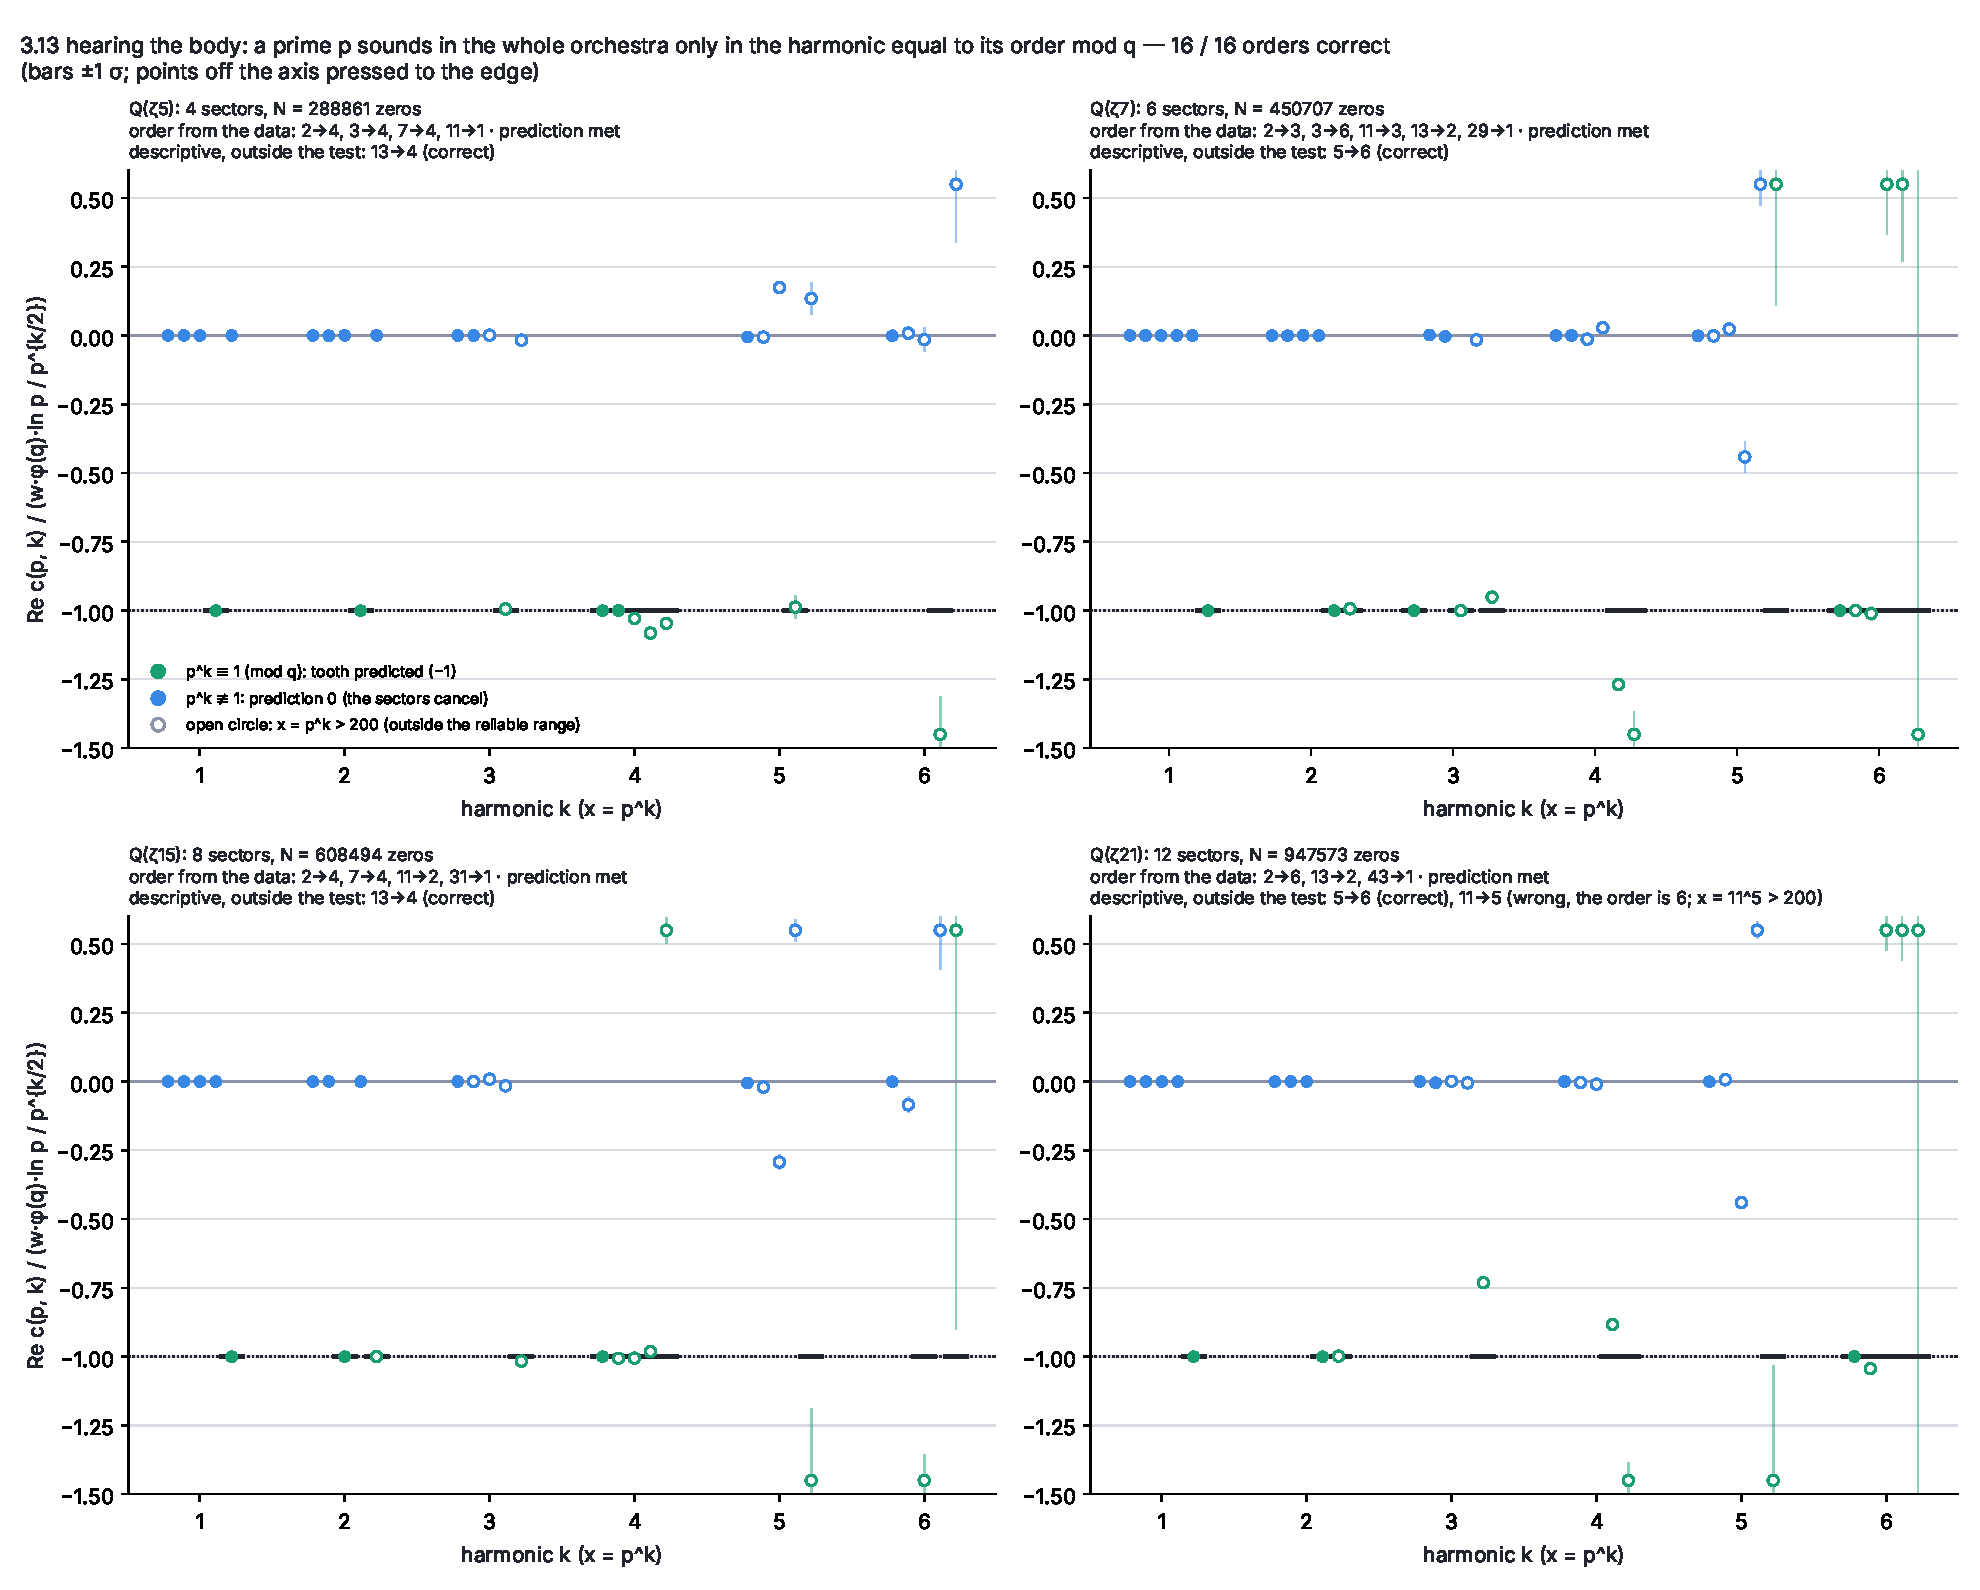
\includegraphics[width=1\textwidth,height=\textheight]{../figures/03_body_en.pdf}
\caption{Figure 3. Hearing the body of the instrument (test 3.13): the
coefficients \(\mathrm{Re}\,c(p, k)\) of the unions of all characters
modulo 5, 7, 15 and 21, normalised to the full strength of a tooth,
against the harmonic \(k\). Filled green: \(p^k \equiv 1 \pmod q\),
predicted \(-1\); filled blue: predicted 0; open circles:
\(x = p^k > 200\), outside the test (\(\pm 1\) error; points beyond the
axis are drawn at its edge).}
\end{figure}

\hypertarget{shared-orbits}{%
\subsection{4.5 Shared orbits}\label{shared-orbits}}

For all 18 pairs of the same modulus the cross-covariance at
\(\ln x = 3\) is 19 times its error and agrees with the prime trace with
the relative phase \(\chi_a(p)\overline{\chi_b(p)}\) to
\(4\cdot10^{-5}\) relative; at \(\ln x = 4, 5, 6\) the relative
difference is at most \(3\cdot10^{-4}\), \(7\cdot10^{-3}\) and
\(3\cdot10^{-2}\), while the expected signal falls to 15, 3.5 and 0.7
times the error. All \(|z| \le 0.06\): the error estimate (the larger of
the independent-window formula and the scatter over sub-bands) is again
conservative, so the agreement is better described by the relative
difference. Near \(\tau = 1\) the largest normalised cross-covariance on
the comb grid is 0.76--0.92 (descriptive).

\hypertarget{saturation}{%
\subsection{4.6 Saturation}\label{saturation}}

The number variance of all fifteen L-functions agrees with the two-point
function without the factors \(p \mid q\): \(Q = 0.32\)--\(1.72\); for
example 21.17: \(\Sigma^2 = 0.317, 0.401, 0.324\) at
\(\ell \approx 1.06, 11.2, 91.1\) against \(0.317, 0.400, 0.324\). GUE
gives \(Q \ge 6{,}500\), the naive prediction \(Q \ge 81\), and Berry's
diagonal formula, which is exact only asymptotically,
\(Q = 11.6\)--\(29.8\) at this height.

\hypertarget{robustness-of-the-main-resonance}{%
\subsection{4.7 Robustness of the main
resonance}\label{robustness-of-the-main-resonance}}

The zeros used in this part (the bands P8 and P3e10 of Platt's tables,
52,498 independent windows each) had already been seen in study VI; only
the numbers below are new, so this part is weaker than a blind test.

\emph{Another window.} With the Hann window the variance at \(\tau = 1\)
is \(1.4330 \pm 0.0063\) in P8 (prediction 1.4305, \(z = +0.40\); GUE
without arithmetic 0.9992, \(z = +69.4\)) and \(1.3943 \pm 0.0061\) in
P3e10 (prediction 1.3897, \(z = +0.76\); GUE \(z = +64.9\)). Over the
201 points of the scan \(Q = 0.66\) and \(0.93\) against the two-point
function and \(737\) and \(531\) against GUE (Fig. 4).

\emph{Other error estimates.} With the Gaussian window of study VI and
six estimates of the error at \(\tau = 1\) (5, 10, 20 and 40 sub-bands,
\(V/\sqrt M\), and a block jackknife with 1,000 blocks) the distance
from GUE is between 13.4 and 69.3 errors in P8 and between 12.0 and 62.2
in P3e10; the distance from the two-point function is at most 0.71 and
0.92. The figure of 46.1 errors quoted in study VI is thus one value
from a range set by the choice of the error estimate. The smallest value
of the range is 12.

\emph{Full covariance.} With the covariance matrix of the 201 points
(block jackknife, Hotelling's correction) the two-point function is
compatible with the data (\(p = 0.976\) and \(0.978\)) and GUE is not
(\(p < 10^{-10}\)). The 201 points are equivalent to 42 and 54
independent points. The largest deviation from the prediction over the
scan is 2.68 and 2.77 errors; allowing for the search over the grid, its
global \(p\)-value is 0.55 and 0.47. At control points away from the
resonances (\(\tau = 0.5\) to \(2.0\)) the deviation from the prediction
is at most 1.71 and 1.05 errors.

\emph{The L-functions.} With the Hann window the combs of the twelve
L-functions of set hr7 and of the three real characters of study VI in
the same band give \(Q = 0.46\)--\(0.86\) against the prediction and
\(14\)--\(55\) against GUE. With the full covariance (364 windows) \(p\)
is between 0.71 and 1.00 for fourteen of the fifteen and 0.042 for the
character modulo 5 with \(\chi(2) = i\) (5.2); the pass mark,
\(p \ge 10^{-3}\) for all twelve, is met, and one value of this size
among fifteen is not unusual.

\begin{figure}
\centering
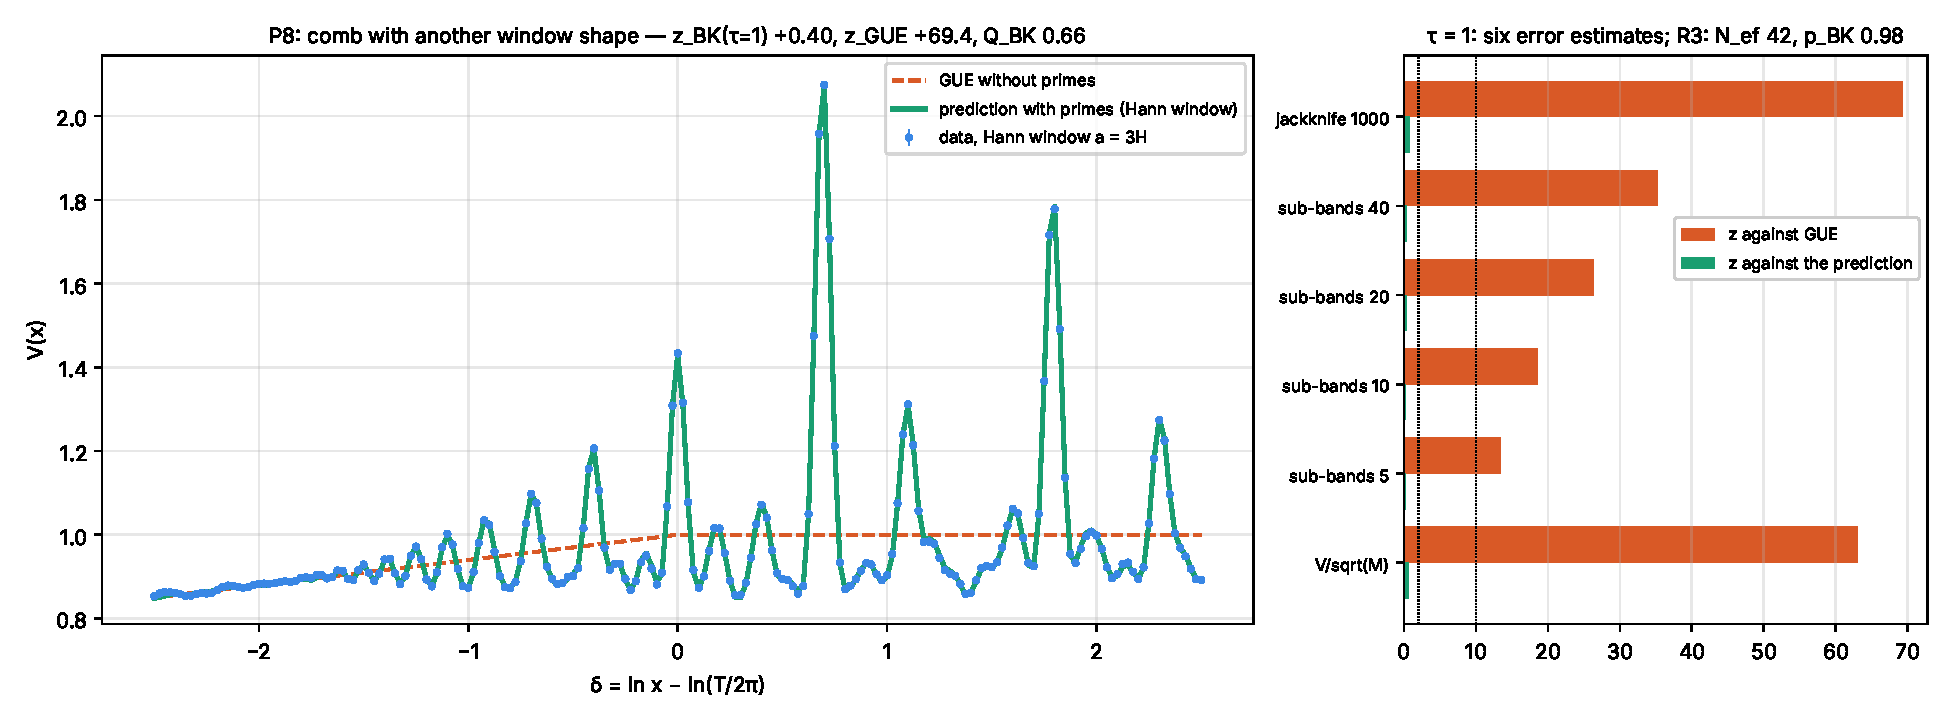
\includegraphics[width=1\textwidth,height=\textheight]{../figures/04a_robustness_P8_en.pdf}
\caption{Figure 4a. Robustness of the main resonance of study VI, band
P8 (\(t \approx 10^8\)). Left: the comb with the Hann window against the
two-point function and GUE without arithmetic. Right: the distance from
GUE and from the prediction at \(\tau = 1\) for the six error
estimates.}
\end{figure}

\begin{figure}
\centering
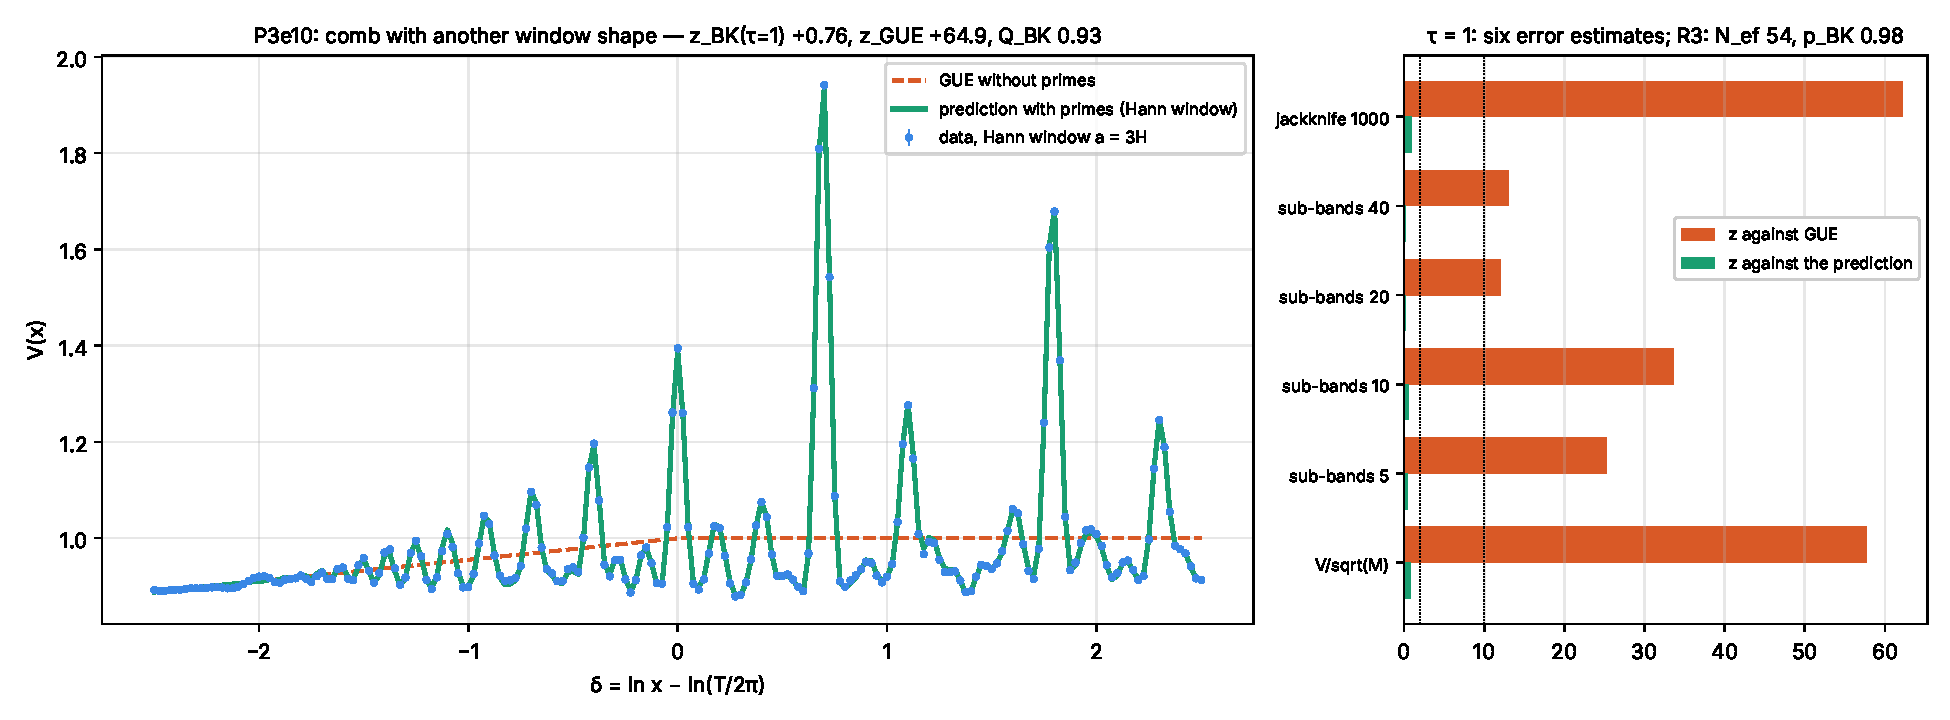
\includegraphics[width=1\textwidth,height=\textheight]{../figures/04b_robustness_P3e10_en.pdf}
\caption{Figure 4b. The same for the band P3e10
(\(t \approx 3\cdot10^{10}\)).}
\end{figure}

\hypertarget{hearing-the-instrument-the-tuning-and-the-body}{%
\subsection{4.8 Hearing the instrument, the tuning and the
body}\label{hearing-the-instrument-the-tuning-and-the-body}}

Three blind tests, specified with their pass marks in addenda 5 and 6
before the data were evaluated, turn the results above into a use. They
are described with the musical reading in Section 5; the numbers are
these. From the first-order coefficients alone the modulus and the
character were identified for 16 of 16 L-functions, with a score of at
most \(1.1\cdot10^{-6}\) against 6.0 or more for the next candidate
(smallest value 5.999) (Section 5.4). From the comb alone the primes
among 2, 3, 5, 7 that divide the modulus were identified for 16 of 16
(\(Q = 0.13\)--\(0.78\), next subset \(2.25\)--\(10.97\); Section 5.5,
Fig. 5). From the union of all characters of a modulus the order of a
prime was read correctly for all 16 primes fixed in advance in four
cyclotomic fields (Section 5.6, Fig. 3).

\begin{figure}
\centering
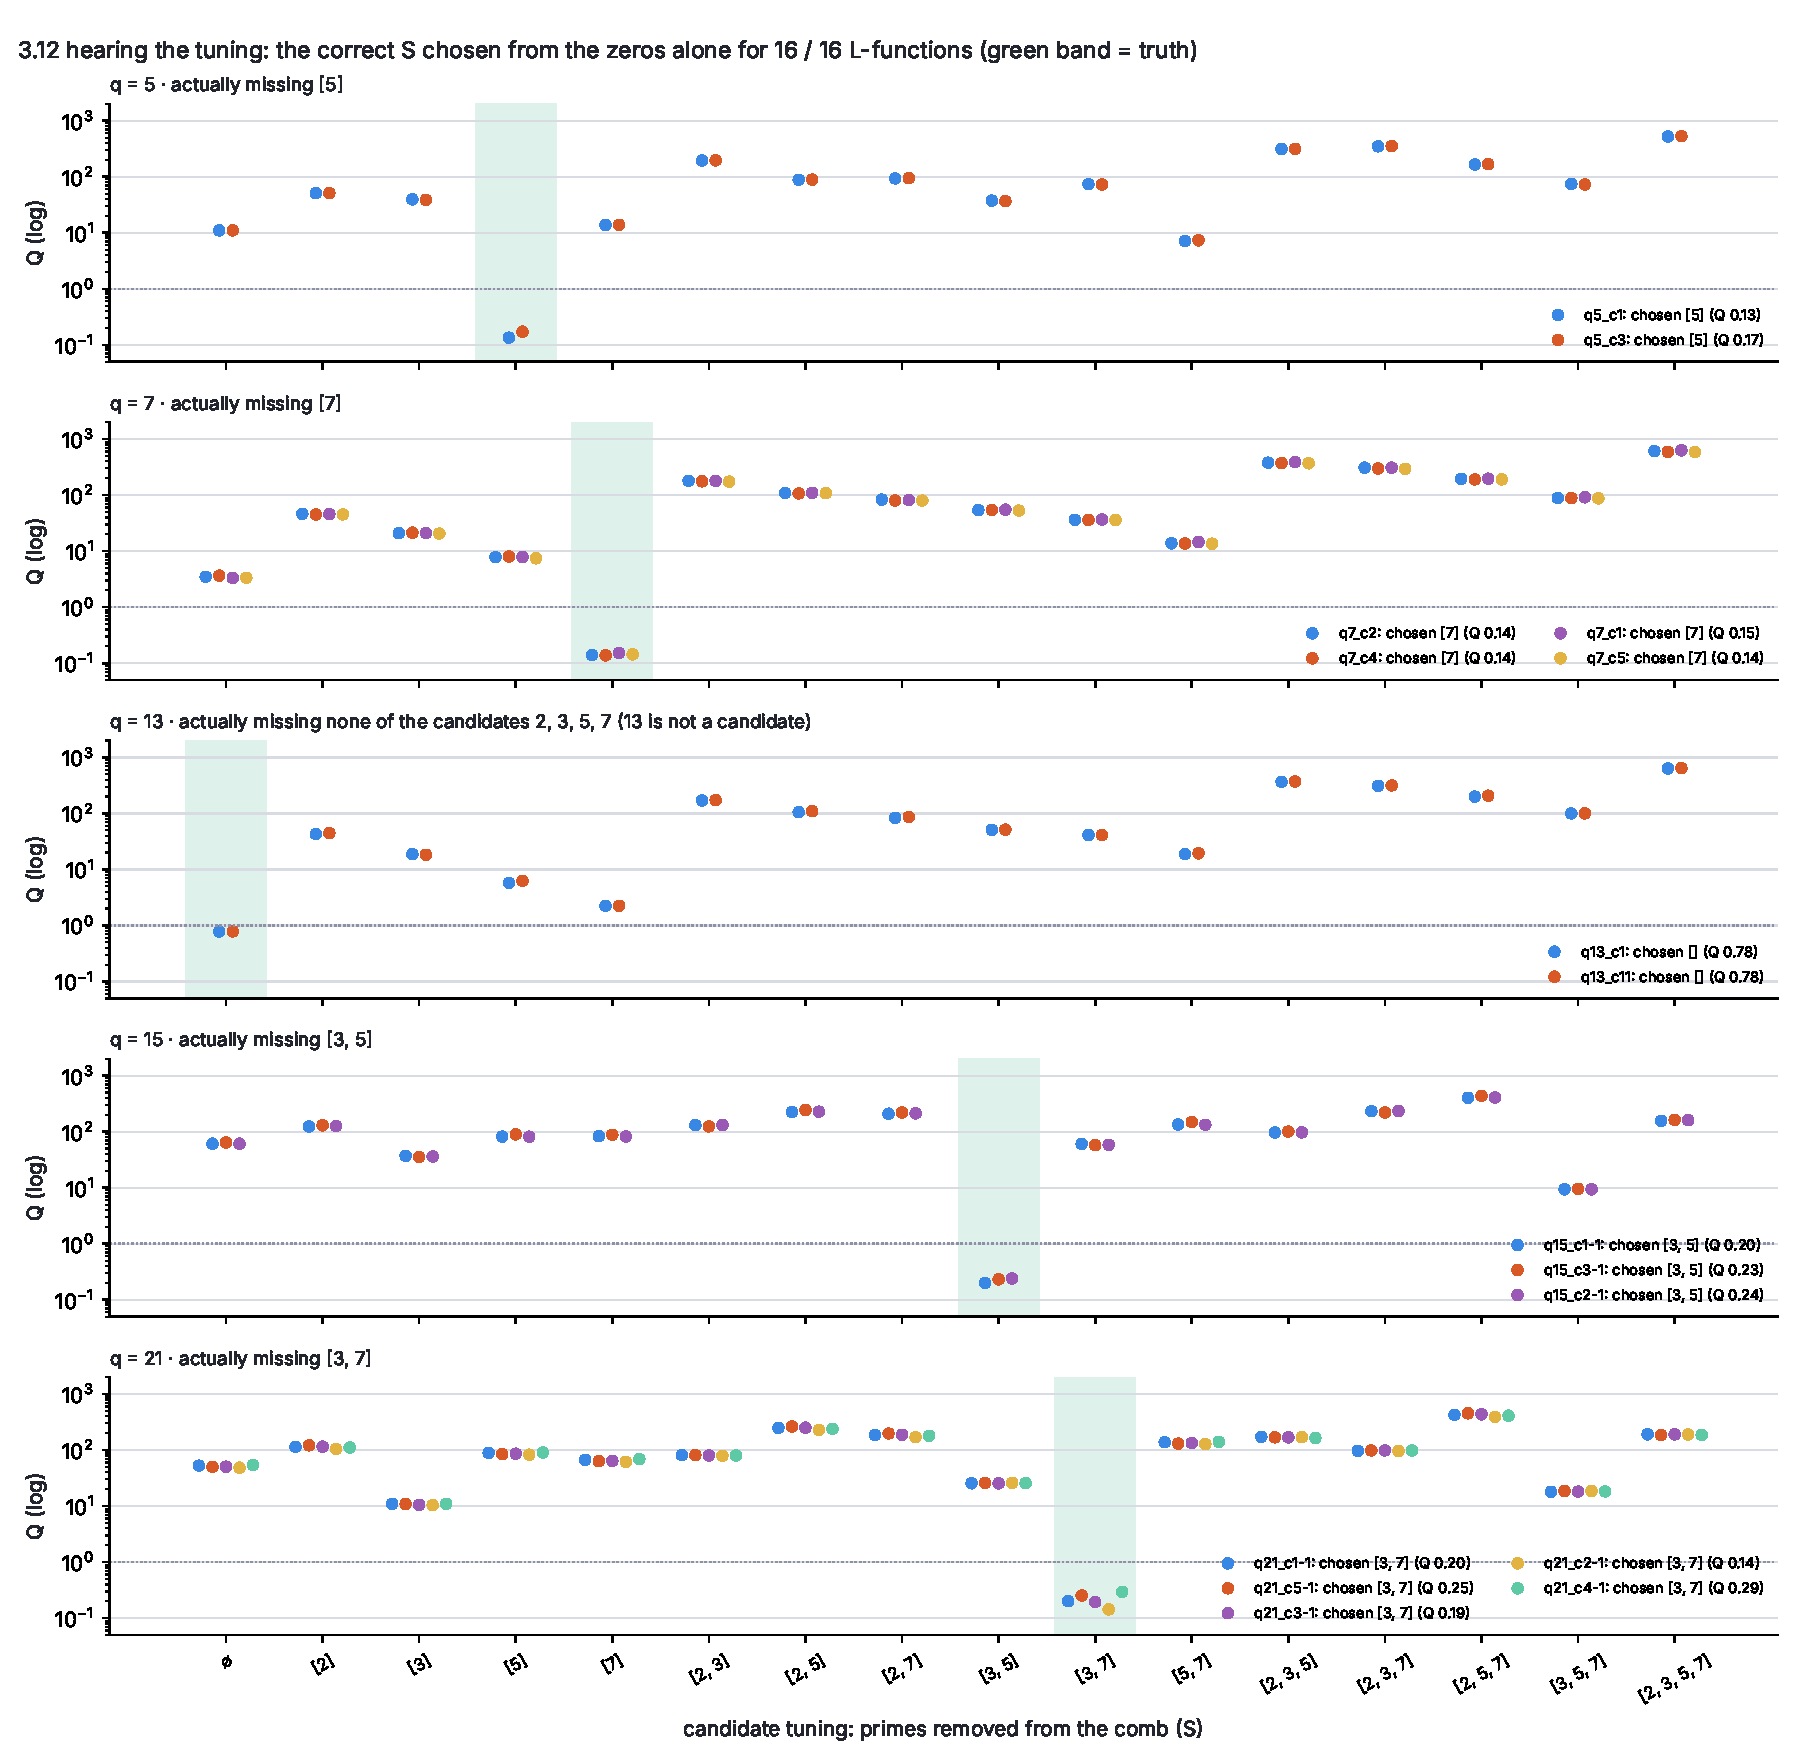
\includegraphics[width=1\textwidth,height=\textheight]{../figures/05_tuning_en.pdf}
\caption{Figure 5. Hearing the tuning (test 3.12): \(Q\) of the comb of
each of the 16 L-functions against the prediction with the primes of a
subset \(S\) of \(\{2, 3, 5, 7\}\) removed; the shaded band marks the
primes that divide the modulus.}
\end{figure}

\hypertarget{certification}{%
\subsection{4.9 Certification}\label{certification}}

Ten windows of each L-function spread over the band (windows starting at
36,000, 40,400, \ldots, 75,600; 120 windows, 21,707 zeros) were
certified with interval arithmetic (Arb through python-flint {[}21{]}):
the sign of the Hardy function \(Z(t, \chi)\) was certified, with
rigorous error bounds, to change between consecutive midpoints, at a
working precision of at most 80 bits, for every zero (check K1). The ten
closest pairs of each L-function in unfolded spacing (120 pairs;
smallest unfolded spacing 0.0071, smallest spacing \(3.9\cdot10^{-3}\))
were separated in the same way (K4). Recomputing two windows of each
L-function (36,000--36,100 and 58,000--58,100) on the desktop computer
in PARI with working precision 38 digits instead of 19 (K2) and with a
four times finer search step (K3) gave the same counts and positions
within \(5.1\cdot10^{-11}\) (48 recomputations for set hr7, 16 for the
four L-functions added for the fields \(\mathbb{Q}(\zeta_{15})\),
\(\mathbb{Q}(\zeta_{21})\)). These checks do not see a pair of very
close zeros missed in another window; for that a count test of Turing
type was added (Section 4.10).

\hypertarget{completeness-two-missed-pairs-of-close-zeros}{%
\subsection{4.10 Completeness: two missed pairs of close
zeros}\label{completeness-two-missed-pairs-of-close-zeros}}

The zeros were found from sign changes of the Hardy function on a grid
of one thirty-second of the mean spacing, with a refinement only when a
window of width 100 fell short of the smooth count by more than 1.5
zeros. Before set hr7b was evaluated, a further test was added (addendum
7 to the rules): with \(r_n = \theta_\chi(\gamma_n)/\pi - n\), a missing
zero shows as a lasting step of \(r_n\) by \(+1\). The mean of \(r_n\)
over the next 400 zeros minus the mean over the previous 400 stays
within 0.01 for all twelve L-functions of set hr7, which are therefore
complete. In set hr7b it showed a step of \(+2.00\) in two windows: a
pair of zeros \(9\cdot10^{-3}\) apart at \(\gamma \approx 62{,}027.74\)
for the character 15.14 and a pair \(1.0\cdot10^{-2}\) apart at
\(\gamma \approx 51{,}751.58\) for 21.11 had been stepped over. The
counts of the two windows were below the smooth count by 1.49 and by
0.95 zeros, so the refinement was not triggered; a deficit of this size
is within the ordinary fluctuation of \(S(t)\), and a count over a
single window cannot detect a missing pair. Both windows were recomputed
on the desktop computer with a four times finer grid: exactly the two
zeros were added in each, no zero changed, and an independent
recomputation in the cloud is identical bit for bit. After the repair no
step remains in any of the 16 L-functions. The tests of Section 5 were
run only then, with one exception stated in Section 5.4.

\hypertarget{resolution-what-the-union-hears-near-115-and-116}{%
\subsection{\texorpdfstring{4.11 Resolution: what the union hears near
\(11^5\) and
\(11^6\)}{4.11 Resolution: what the union hears near 11\^{}5 and 11\^{}6}}\label{resolution-what-the-union-hears-near-115-and-116}}

This analysis was made after the evaluation (addendum 8 to the rules)
and is descriptive. A sum over the zeros of a band of width \(\Delta T\)
separates two numbers \(x\) and \(x + d\) only if
\(d \gtrsim 2\pi x/\Delta T \approx x/7000\): 0.03 at \(x = 200\), but
23 at \(11^5\) and 253 at \(11^6\). In the union modulo 21 every prime
power \(n \equiv 1 \pmod{21}\) sounds with weight
\(\varphi(21)\Lambda(n)/\sqrt n\), and the prime 161,071 \(\equiv 1\)
lies 20 above \(11^5 = 161{,}051 \equiv 2\). With a Gaussian weight over
the whole band (\(T_0 = 58{,}000\), \(H = 4{,}000\)) the sum
\(Z(x) = \sum_\gamma g(\gamma)x^{i\gamma}\) over the 947,573 zeros of
the union was compared with the explicit formula summed over the prime
powers near \(x\), without a free parameter, at \(11^k\) (\(k \le 6\))
and on 1,602 points around \(11^5\) and \(11^6\) (Fig. 6): they agree to
\(1.9\cdot10^{-10}\) of the total weight, that is to \(1.2\cdot10^{-6}\)
of the full strength of a tooth of 11. At \(11^5\) the measured value is
4.42 times that strength and comes entirely from 161,071; once the
neighbouring primes are subtracted the remainder is \(2\cdot10^{-7}\),
so 11 is silent in the fifth harmonic, as it must be. At
\(11^6 = 1{,}771{,}561 \equiv 1\) the tooth of 11 is buried under the
primes \(\equiv 1 \pmod{21}\) around it (55 within 5,800, the nearest
126 away); after subtracting them the remainder is \(-1.000001\), the
tooth of 11 at full strength. The subtraction uses the list of primes,
so it is a check of the explicit formula and not a reading from the
zeros alone.

Near \(11^5\) a reading from the zeros and the modulus alone is still
possible, because the width of the kernel (40) is comparable with the
spacing of the odd candidates \(n \equiv 1 \pmod{21}\) (42): a
least-squares fit of unknown amplitudes at these candidates and of a
trial term at \(11^5\) itself (29 unknowns, condition number
\(1.8\cdot10^7\)) returns the amplitude of the trial term as
\(3\cdot10^{-6}\) of the full strength, and among the 14 candidates
within 300 of \(11^5\) it returns the five primes with amplitude
\(1 \pm 4\cdot10^{-7}\) and the nine composite numbers with at most
\(5\cdot10^{-7}\). At \(11^6\) the kernel is ten times wider than the
spacing and no such reading is possible in this band; reading the order
6 from the zeros alone would need a band about ten times wider.

\begin{figure}
\centering
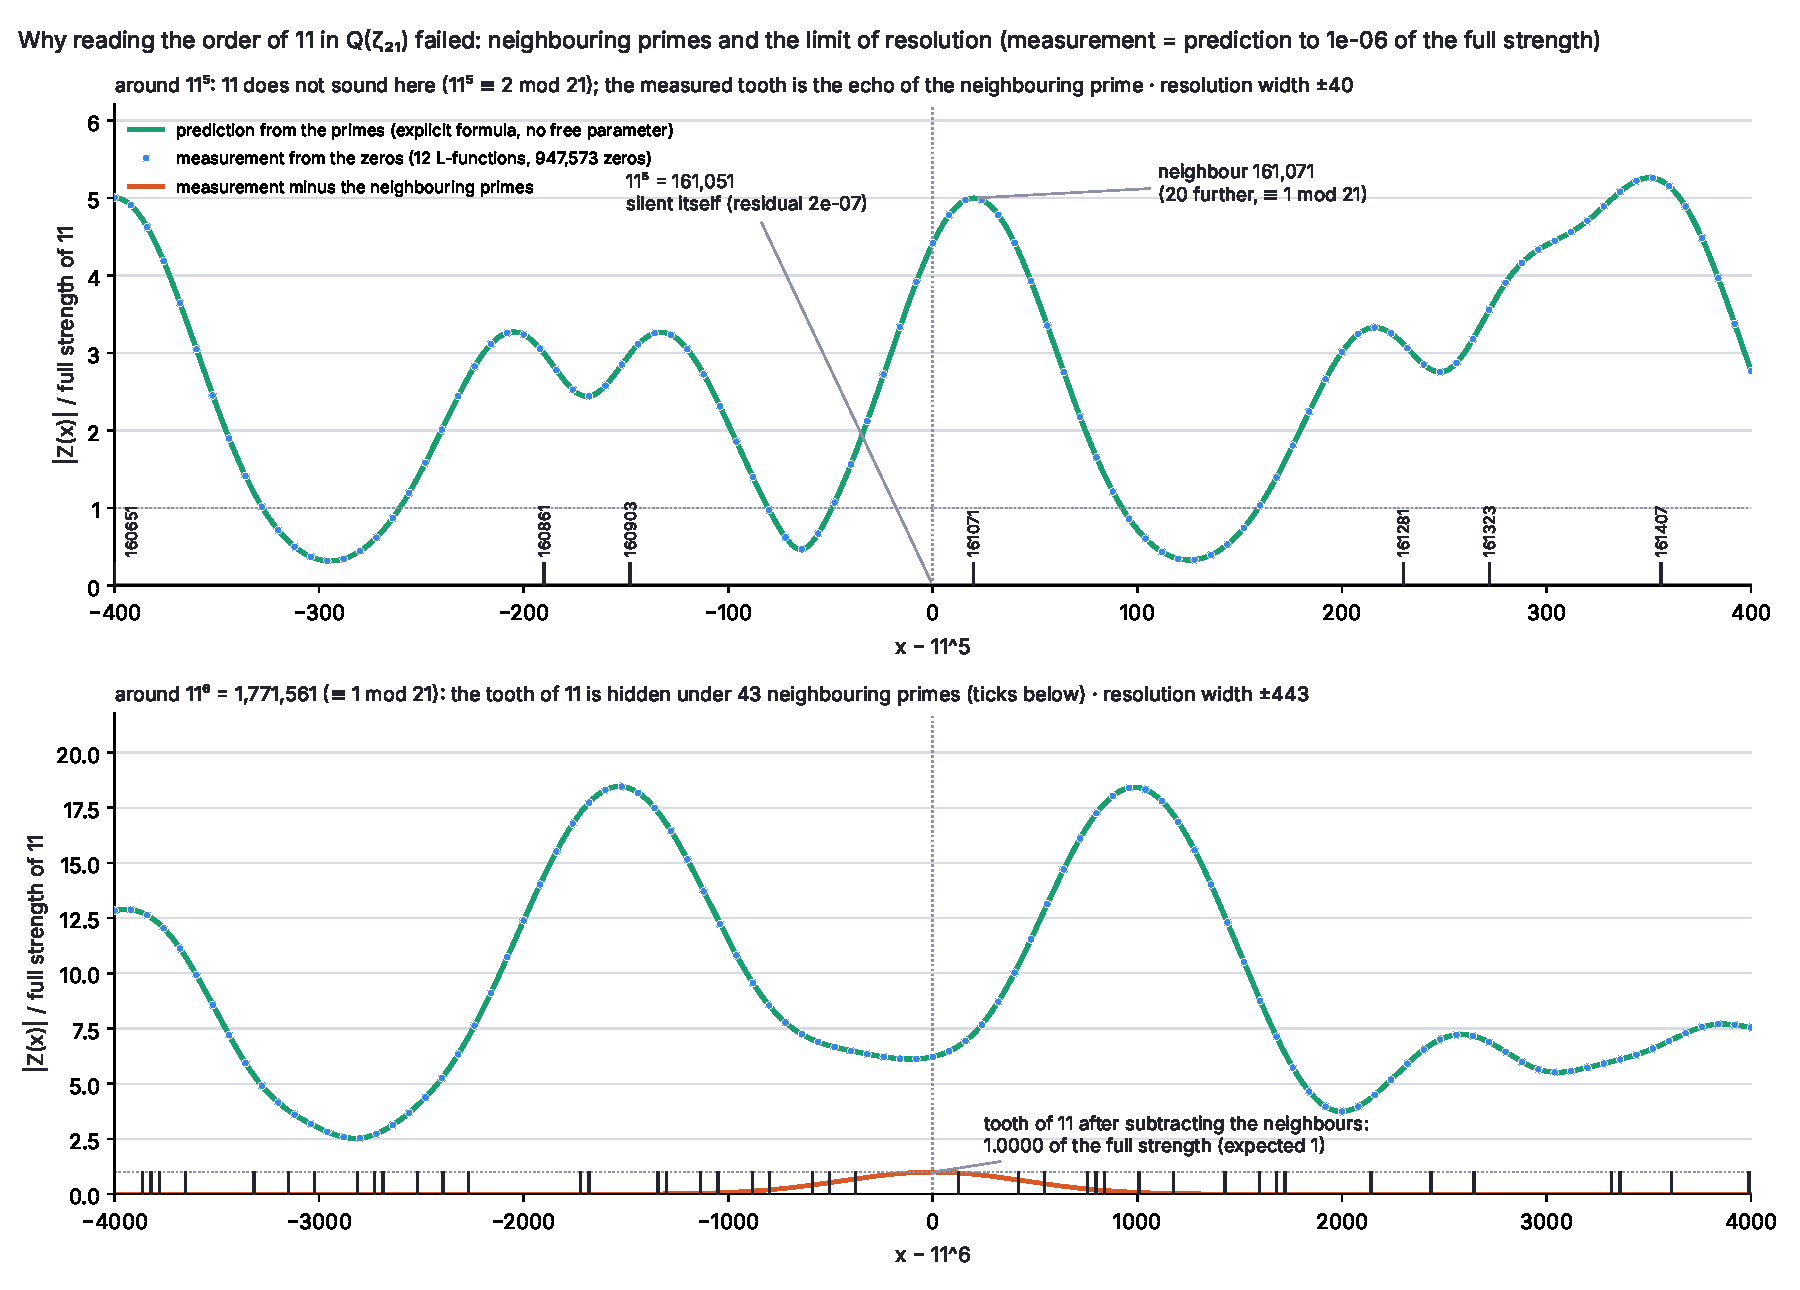
\includegraphics[width=1\textwidth,height=\textheight]{../figures/06_resolution_en.pdf}
\caption{Figure 6. Resolution near \(11^5\) and \(11^6\) in the union
modulo 21: \(|Z(x)|\) from the 947,573 zeros of the union (points)
against the explicit formula summed over the prime powers near \(x\)
(line), in units of the full strength of a tooth of 11, and the
remainder after the neighbouring primes are subtracted; ticks mark the
primes \(\equiv 1 \pmod{21}\).}
\end{figure}

\hypertarget{where-random-matrices-end-the-pair-correlation-of-one-l-function}{%
\subsection{4.12 Where random matrices end: the pair correlation of one
L-function}\label{where-random-matrices-end-the-pair-correlation-of-one-l-function}}

For all 16 L-functions the pair correlation up to three mean spacings is
described by the two-point function of {[}8{]}: \(\chi^2\) per bin
0.78--1.86 against the pass mark 2.0. The GUE form alone gives
6.3--16.5. At half a mean spacing the measured \(R_2\) lies below the
GUE value by 0.032--0.076; the prediction is 0.045--0.065, depending on
the modulus. The largest deviation of a single bin from the prediction
is 2.3--4.0 errors. At this height the random-matrix form alone is
therefore visibly incomplete already at the shortest distances, and the
arithmetic correction accounts for the difference (Fig. 7).

Descriptively, the nearest-neighbour spacing distribution of the
1,296,642 spacings of all 16 L-functions together differs from the GUE
distribution by up to 0.083 (at \(s = 1.15\)): there are fewer small
spacings (\(-0.06\) near \(s = 0.45\)), more spacings near the mean
(\(+0.08\) near \(s = 1.0\)--\(1.2\)) and fewer large ones (\(-0.03\)
near \(s = 1.8\)). The spectrum is stiffer than GUE. No unitary matrix
size reproduces the distribution within the errors: \(\chi^2\) per bin
is 156 for \(N = 3\), 304 for \(N = 4\), 1,931 for \(N = 2\) and 1,180
for GUE, while the effective size read from the predicted \(R_2\) near
zero is 2.0--2.3. At \(\ln(q\gamma/2\pi) \approx 11\)--\(12\) a single
effective matrix size is thus not an adequate description of the
spacings; the two-point theory is adequate for the pair correlation.
(\(\chi^2\) values of the spacing distribution for individual
L-functions are not quoted: some bins have zero block variance.)

\begin{figure}
\centering
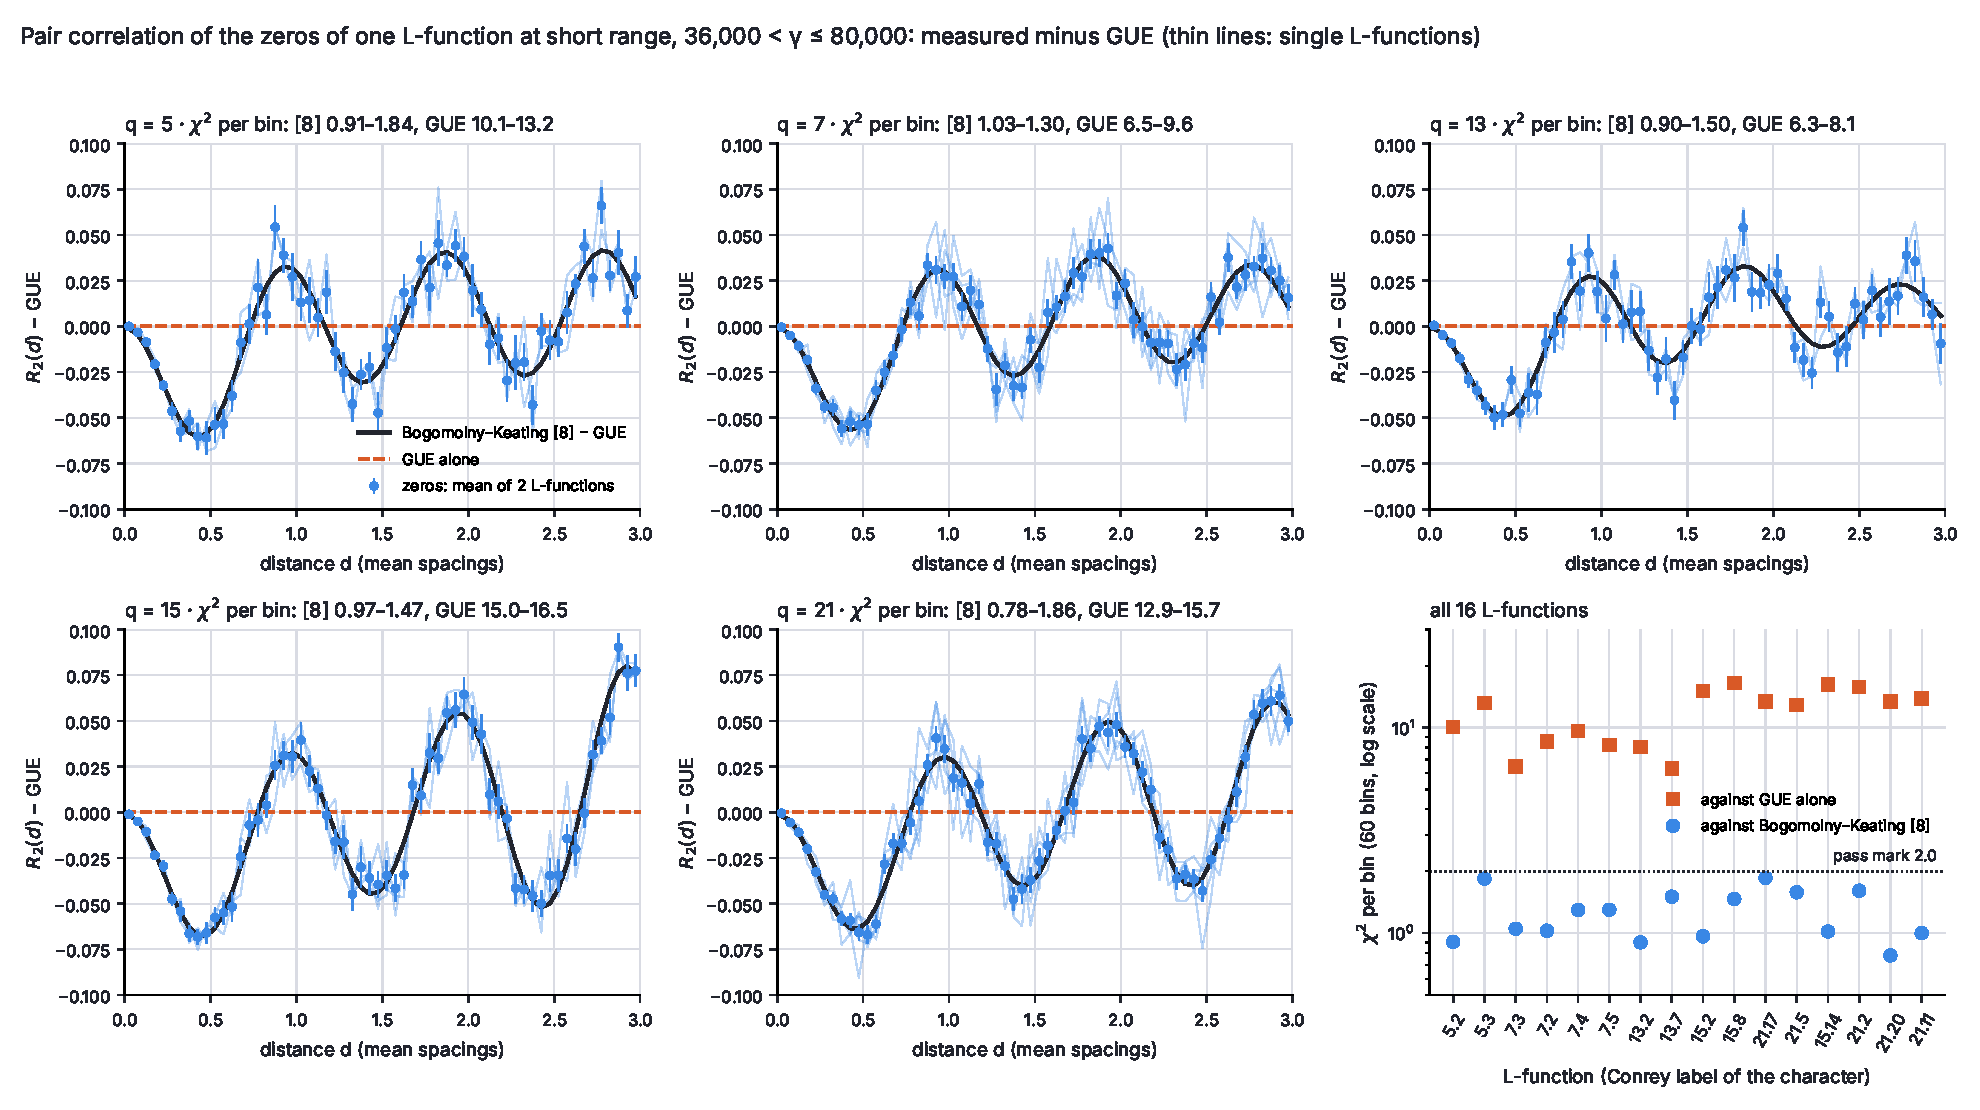
\includegraphics[width=1\textwidth,height=\textheight]{../figures/07_pair_correlation_en.pdf}
\caption{Figure 7. Pair correlation of single L-functions minus the GUE
form, \(36{,}000 < \gamma \le 80{,}000\): data (\(\pm 1\) error) against
the two-point function of {[}8{]}, by modulus (thin lines: single
L-functions). Lower right: \(\chi^2\) per bin of all 16 L-functions
against {[}8{]} and against GUE alone, with the pass mark.}
\end{figure}

\hypertarget{the-orchestra-as-a-superposition-of-independent-spectra}{%
\subsection{4.13 The orchestra as a superposition of independent
spectra}\label{the-orchestra-as-a-superposition-of-independent-spectra}}

{\small\begin{longtable}[]{@{}
  >{\raggedright\arraybackslash}p{(\columnwidth - 14\tabcolsep) * \real{0.1486}}
  >{\raggedright\arraybackslash}p{(\columnwidth - 14\tabcolsep) * \real{0.0676}}
  >{\raggedright\arraybackslash}p{(\columnwidth - 14\tabcolsep) * \real{0.1081}}
  >{\raggedright\arraybackslash}p{(\columnwidth - 14\tabcolsep) * \real{0.0946}}
  >{\raggedright\arraybackslash}p{(\columnwidth - 14\tabcolsep) * \real{0.2973}}
  >{\raggedright\arraybackslash}p{(\columnwidth - 14\tabcolsep) * \real{0.0946}}
  >{\raggedright\arraybackslash}p{(\columnwidth - 14\tabcolsep) * \real{0.0946}}
  >{\raggedright\arraybackslash}p{(\columnwidth - 14\tabcolsep) * \real{0.0946}}@{}}
\toprule\noalign{}
\begin{minipage}[b]{\linewidth}\raggedright
union
\end{minipage} & \begin{minipage}[b]{\linewidth}\raggedright
sectors
\end{minipage} & \begin{minipage}[b]{\linewidth}\raggedright
zeros
\end{minipage} & \begin{minipage}[b]{\linewidth}\raggedright
largest \(|p - p_S|\)
\end{minipage} & \begin{minipage}[b]{\linewidth}\raggedright
first bin: measured / \(p_S\) / Poisson
\end{minipage} & \begin{minipage}[b]{\linewidth}\raggedright
largest distance from one GUE
\end{minipage} & \begin{minipage}[b]{\linewidth}\raggedright
\(\chi^2\) per bin against \(p_S\)
\end{minipage} & \begin{minipage}[b]{\linewidth}\raggedright
bins beyond 3 errors (of 40)
\end{minipage} \\
\midrule\noalign{}
\endhead
\bottomrule\noalign{}
\endlastfoot
\(\mathbb{Q}(\zeta_5)\) & 4 & 288,861 & 0.0096 & 0.721 / 0.731 / 0.952 &
0.71 & 3.4 & 3 \\ \addlinespace[2pt]
\(\mathbb{Q}(\zeta_7)\) & 6 & 450,707 & 0.0075 & 0.798 / 0.805 / 0.952 &
0.79 & 4.9 & 3 \\ \addlinespace[2pt]
\(\mathbb{Q}(\zeta_{15})\) & 8 & 608,494 & 0.0068 & 0.837 / 0.842 /
0.952 & 0.83 & 3.2 & 2 \\ \addlinespace[2pt]
\(\mathbb{Q}(\zeta_{21})\) & 12 & 947,573 & 0.0073 & 0.872 / 0.879 /
0.952 & 0.86 & 1.9 & 0 \\ \addlinespace[2pt]
\end{longtable}}

All three pass marks are met for all four unions: the zeros of a
cyclotomic Dedekind zeta function in this band are spaced like a
superposition of independent GUE spectra, one for each character, and
neither like a single GUE spectrum nor like a Poisson process (Fig. 8),
as expected from {[}30{]} and {[}24{]}. The agreement is not perfect.
\(\chi^2\) per bin against \(p_S\) is 1.9--4.9 and the largest single
deviation is 2.9--8.3 errors; in the first bin the measured density is
below \(p_S\) in all four unions, by 0.006--0.010. The smallest spacings
are thus slightly rarer than independent spectra would give. The sign is
the one suggested by the cross-covariance of Section 4.5 (the sectors of
one modulus share their primes), but the size of this effect was not
computed and no claim is made about it. The model \(p_S\) is insensitive
to the height within the band (at most 0.0002).

\begin{figure}
\centering
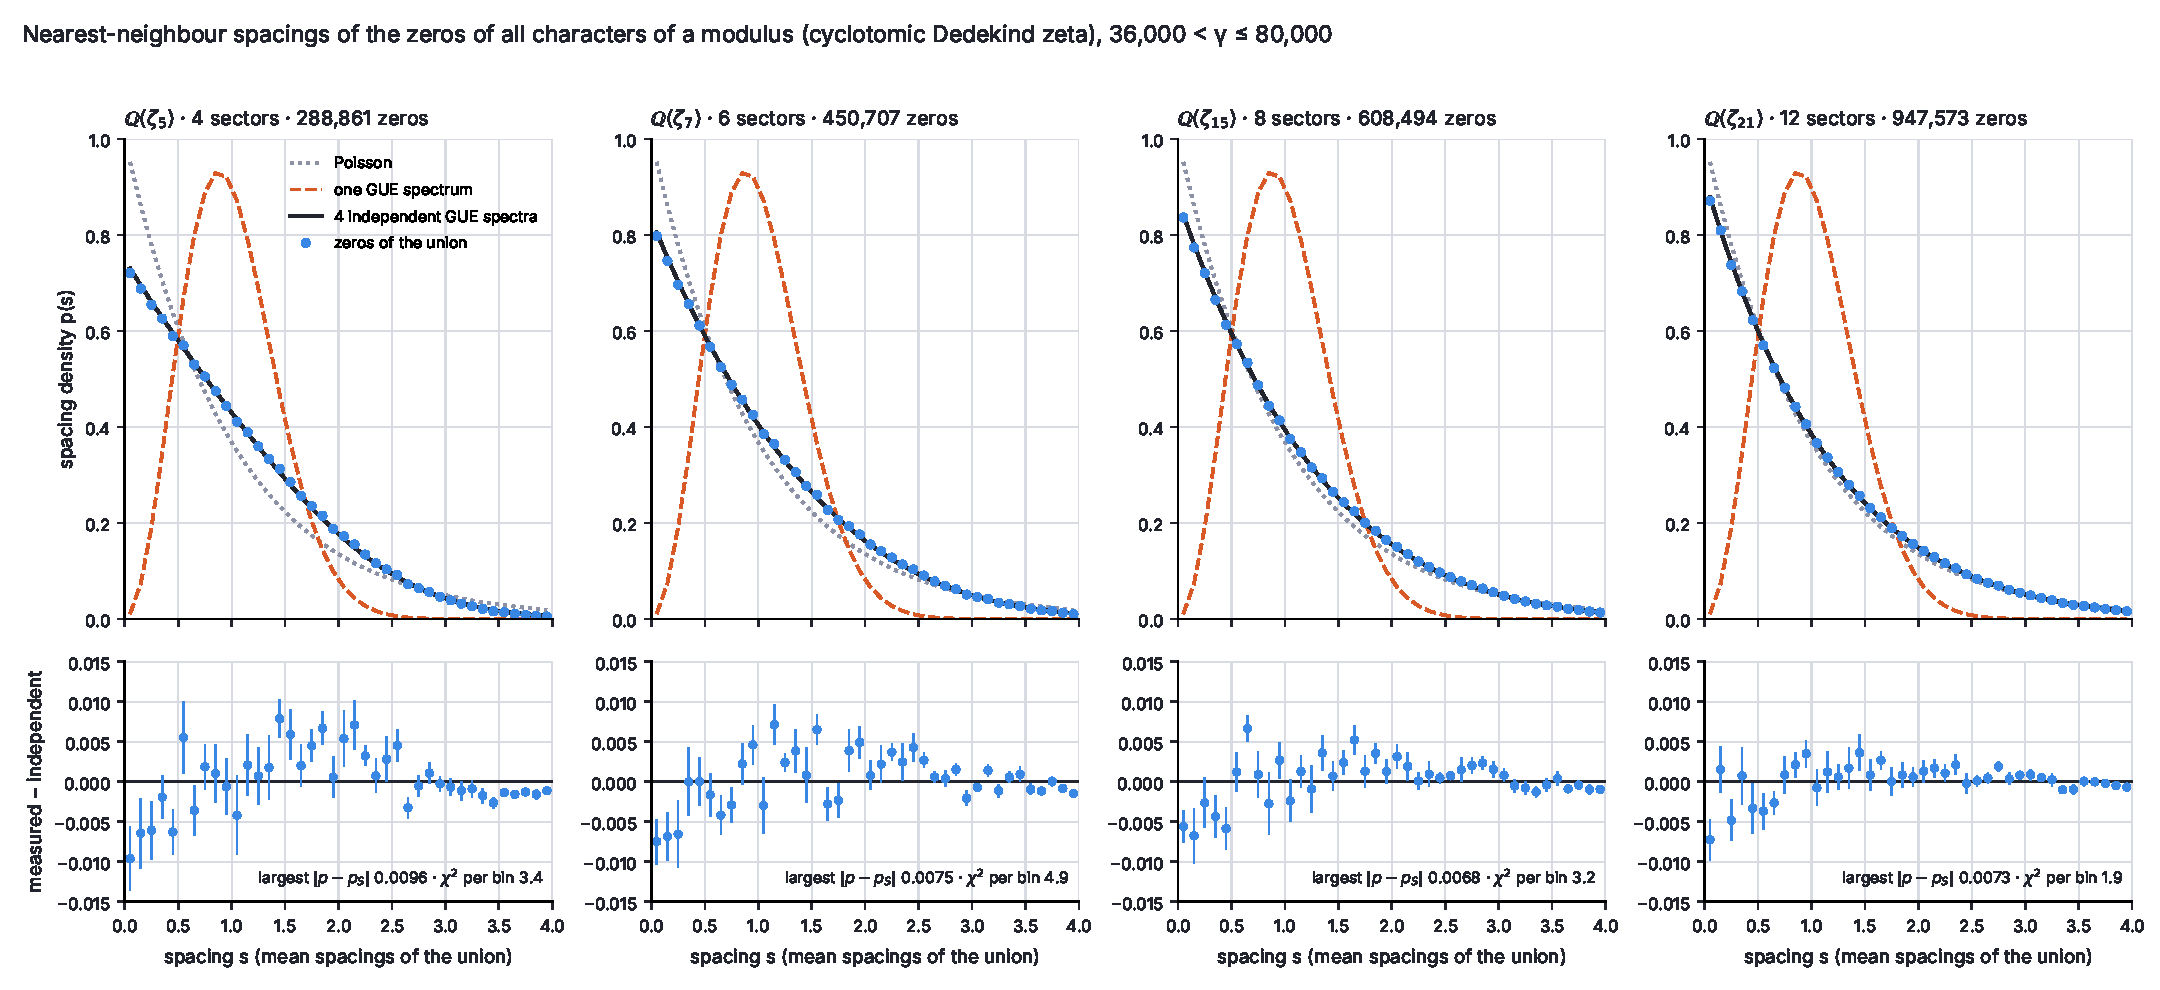
\includegraphics[width=1\textwidth,height=\textheight]{../figures/08_unions_en.pdf}
\caption{Figure 8. Spacing densities of the four unions (the zeros of
the Dedekind zeta functions of \(\mathbb{Q}(\zeta_5)\),
\(\mathbb{Q}(\zeta_7)\), \(\mathbb{Q}(\zeta_{15})\),
\(\mathbb{Q}(\zeta_{21})\)) against the superposition of independent GUE
spectra, a single GUE spectrum and a Poisson process; lower panels: the
measured density minus the superposition (\(\pm 1\) error).}
\end{figure}

\hypertarget{height-does-the-deviation-from-random-matrices-fade-as-predicted}{%
\subsection{4.14 Height: does the deviation from random matrices fade as
predicted?}\label{height-does-the-deviation-from-random-matrices-fade-as-predicted}}

In the second band, \(400{,}000 < \gamma \le 420{,}000\), the four
L-functions of set hr7b have 43,907 to 44,980 zeros, 178,844 in total.
The counts differ from the smooth count by \(-0.65\) to \(+1.35\), and
the count test of Section 4.10 shows no step (largest \(|\Delta|\)
0.01). Six zeros of each L-function chosen at random (24 in all) give
\(|L(\tfrac12 + i\gamma, \chi)| \le 5.4\cdot10^{-9}\) in mpmath, against
at least 0.21 at the midpoints to the next zero.

The pair correlation in this band again follows the two-point function
of {[}8{]}: \(\chi^2\) per bin 1.05--1.82, against 3.5--8.0 for GUE
alone (Fig. 9). The amplitude of the measured deviation from GUE along
the predicted shape is 0.92--1.07 for the four L-functions,
\(0.987 \pm 0.027\) pooled (1 means exactly as predicted;
\(0.995 \pm 0.011\) in the lower band). The size of the deviation falls
from \(0.0363 \pm 0.0004\) in the lower band to \(0.0261 \pm 0.0007\) in
the upper band, 12.6 errors apart. The ratio of the two sizes is
\(0.719 \pm 0.021\); the prediction, with no free parameter, is 0.727.
All four pass marks are met. Between \(L = \ln(qT/2\pi) \approx 12.2\)
and \(14.1\) (for \(q = 21\)) the deviation thus shrinks roughly like
\(1/L^2\), as the two-point function says, and its shape stays the same.
Descriptively, the largest difference of the nearest-neighbour spacing
distribution from GUE is 0.071--0.081 in the upper band and 0.082--0.106
in the lower band for the same four L-functions.

\begin{figure}
\centering
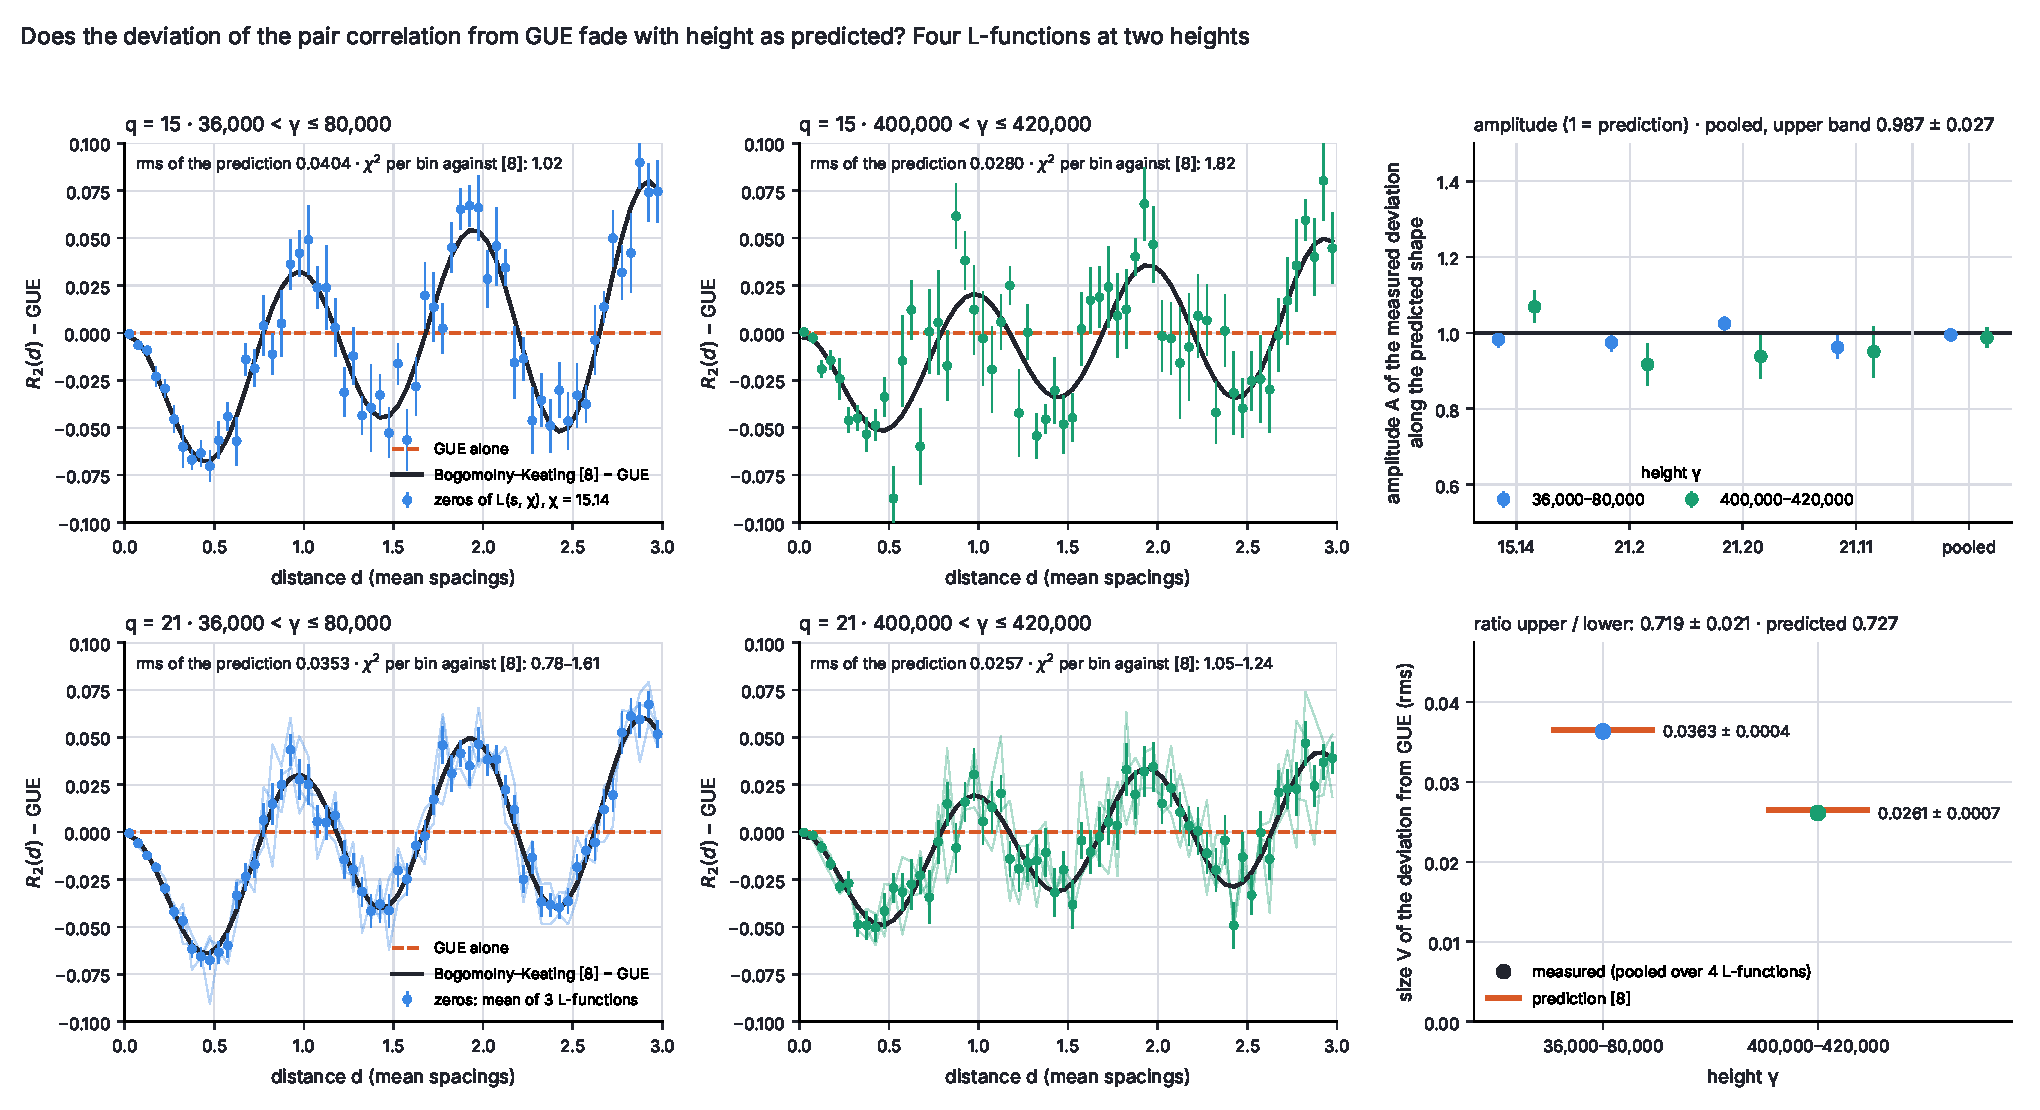
\includegraphics[width=1\textwidth,height=\textheight]{../figures/09_height_en.pdf}
\caption{Figure 9. Height. The pair correlation minus GUE for the
L-functions of set hr7b in the bands 36,000--80,000 and 400,000--420,000
against the two-point function of {[}8{]}; the amplitude of the measured
deviation along the predicted shape for each L-function and pooled; the
size of the deviation in both bands against the prediction.}
\end{figure}

\hypertarget{a-musical-reading-and-how-to-use-it}{%
\section{5. A musical reading, and how to use
it}\label{a-musical-reading-and-how-to-use-it}}

The language of music is used in this series as an aid to reading the
measurements, not as a claim about sound. Each statement below has an
exact counterpart in the formulas of Section 3, and each ``hearing''
test was specified, with its pass mark, before the data were evaluated.

\hypertarget{the-harmonic-series}{%
\subsection{5.1 The harmonic series}\label{the-harmonic-series}}

A string sounds at a fundamental frequency and at its integer multiples,
the overtones. In the explicit formula the primes play the part of
fundamental tones with ``lengths'' \(\ln p\), and the prime powers
\(p^k\) are their overtones with lengths \(k\ln p\) and weights
\(\ln p/p^{k/2}\). The first-order coefficients \(c_k(p)\) of Section
4.4 are literally the amplitudes of these overtones in the zeros.

\hypertarget{the-prime-limit}{%
\subsection{5.2 The prime limit}\label{the-prime-limit}}

In just intonation a tuning is called \(P\)-limit when all its intervals
are ratios of integers built from primes \(\le P\): 3-limit is
Pythagorean tuning, 5-limit adds the pure major third 5/4. The comb of
\(\zeta\) contains the intervals \(A/B\) of all primes; the comb of
\(L(s, \chi)\) lacks exactly the primes dividing \(q\). Modulus 15 is
therefore a tuning without 3 and 5, and its tooth at the octave
\(A/B = 2\) is almost twice as high as for \(q = 5\) (7.15 against 3.81
predicted, 7.13 measured on average), because the octave no longer
shares its strength with the neighbouring intervals built from 3 and 5.
Descriptively, the agreement of the comb improves as more primes are
admitted into the prediction: for \(q = 5\) (5.2), \(Q = 3.3\) with the
prime 2 alone, 0.26 with 2 and 3, and 0.13 with all primes; for
\(q = 15\) (15.2), 0.49 up to \(P = 5\) (only 2 contributes), 0.31 with
7 and 0.20 with all; for \(q = 21\) (21.17), 1.0 up to \(P = 3\), 0.21
from \(P = 5\) and 0.20 with all.

\hypertarget{the-comma}{%
\subsection{5.3 The comma}\label{the-comma}}

Twelve pure fifths overshoot seven octaves by the Pythagorean comma
\(3^{12}/2^{19} \approx 1.0136\); no power of 3 equals a power of 2
because \(\ln 3/\ln 2\) is irrational. In the comb this is why the teeth
sit only at rational ratios \(A/B\): two different prime powers never
have the same length, so the orbits do not merge into a common tooth.
Study VI used irrational multiples as a control: for
\(\alpha = \sqrt2/2\pi\) and \(\sqrt3/2\pi\) the fractional parts
\(\{\gamma\alpha\}\) showed no structure beyond the uniform density
{[}6{]}. No new measurement is made here.

\hypertarget{hearing-the-instrument-test-3.11}{%
\subsection{5.4 Hearing the instrument (test
3.11)}\label{hearing-the-instrument-test-3.11}}

\textbf{Use:} given only a list of zeros, determine which L-function
they belong to. From the first-order coefficients alone, the primes with
\(|c_p| < 0.5\,w\ln p/\sqrt p\) are taken as divisors of the modulus;
among all primitive characters of moduli \(q' \le 30\) with these prime
divisors, the one closest to \(\hat\chi(p) = -c_p\sqrt p/(w\ln p)\) is
chosen. All twelve L-functions of set hr7 were identified correctly,
modulus and character, and so were the four L-functions of set hr7b: 16
of 16, with a score of at most \(1.1\cdot10^{-6}\) against 6.0 or more
for the next candidate (smallest value 5.999). For the four L-functions
of hr7b this result had already been seen on the data before two missing
pairs of zeros were repaired (Section 4.10); it is the same after the
repair.

\hypertarget{hearing-the-tuning-test-3.12}{%
\subsection{5.5 Hearing the tuning (test
3.12)}\label{hearing-the-tuning-test-3.12}}

\textbf{Use:} from the comb alone, without the first order, determine
which small primes divide the modulus. Of the 16 subsets of
\(\{2, 3, 5, 7\}\), the one whose prediction fits the comb best was the
correct one for all 16 L-functions (\(Q = 0.13\)--\(0.78\), next subset
\(Q = 2.25\)--\(10.97\); Fig. 5). For \(q = 15\) the comb itself says
``3 and 5 are missing'', for \(q = 21\) ``3 and 7''.

\hypertarget{hearing-the-body-of-the-instrument-test-3.13}{%
\subsection{5.6 Hearing the body of the instrument (test
3.13)}\label{hearing-the-body-of-the-instrument-test-3.13}}

\textbf{Use:} from the zeros of the whole family of a modulus --- the
orchestra --- read how primes split in the cyclotomic field. In the
union, a prime \(p\) is silent in all harmonics except the multiples of
its order \(f(p)\) modulo \(q\), where it sounds with the full weight
\(\varphi(q)\): the sectors cancel each other everywhere else. The order
read from the data agreed with the arithmetic order for all 16 primes
fixed in advance in the four fields \(\mathbb{Q}(\zeta_5)\),
\(\mathbb{Q}(\zeta_7)\), \(\mathbb{Q}(\zeta_{15})\),
\(\mathbb{Q}(\zeta_{21})\) (Fig. 3; Section 4.4 gives the one wrong
reading outside the test). Removing one sector breaks the cancellation
(negative control, descriptive). How far this hearing reaches is set by
the length of the listening: two tones a frequency difference
\(\Delta f\) apart can be told apart only after a time of about
\(1/\Delta f\), and two numbers \(x\) and \(x + d\) only from zeros over
a height range of about \(2\pi x/d\) (Section 4.11). With the band used
here every integer up to several thousand is resolved; at \(11^5\) the
union can no longer tell 11 from the prime twenty steps away unless the
spacing of the candidates is used, and at \(11^6\) not at all.

\hypertarget{limits-of-the-analogy}{%
\subsection{5.7 Limits of the analogy}\label{limits-of-the-analogy}}

The zeros are not frequencies of a known physical system, and nothing
here is audible without an arbitrary choice of how to turn numbers into
sound. Every effect described in this section follows from theorems ---
the explicit formula, Landau's formula, the orthogonality of characters
and the splitting of primes in cyclotomic fields --- or from the
conjectured two-point function, and the musical words add no new
content. What the blind tests add is practical: the comb and the first
order are enough to recognise an L-function, its modulus and the
splitting of primes from its zeros, which can serve as a check of
computed tables of zeros and as a set of conditions that any proposed
operator for these zeros would have to meet.

\hypertarget{statements-and-their-status}{%
\section{6. Statements and their
status}\label{statements-and-their-status}}

Verdicts as defined in the rules: O = supported (all pass marks met), N
= undecided, Z = rejected.

{\small\begin{longtable}[]{@{}
  >{\raggedright\arraybackslash}p{(\columnwidth - 4\tabcolsep) * \real{0.7692}}
  >{\raggedright\arraybackslash}p{(\columnwidth - 4\tabcolsep) * \real{0.1154}}
  >{\raggedright\arraybackslash}p{(\columnwidth - 4\tabcolsep) * \real{0.1154}}@{}}
\toprule\noalign{}
\begin{minipage}[b]{\linewidth}\raggedright
Statement
\end{minipage} & \begin{minipage}[b]{\linewidth}\raggedright
Section
\end{minipage} & \begin{minipage}[b]{\linewidth}\raggedright
Verdict
\end{minipage} \\
\midrule\noalign{}
\endhead
\bottomrule\noalign{}
\endlastfoot
odv-hr7-hreben: the comb of one \(L(s, \chi)\) follows the modulus & 4.2
& O \\ \addlinespace[2pt]
odv-hr7-nastroje: same modulus, same comb (no theory) & 4.2 & O \\ \addlinespace[2pt]
odv-hr7-faze: the first order carries the phase of \(\chi(p)\) & 4.3 &
O \\ \addlinespace[2pt]
odv-hr7-presne: explicit formula with a Gaussian window (data quality) &
4.3 & O \\ \addlinespace[2pt]
odv-hr7-diag: variance of harmonics in the diagonal regime & 4.3 & O \\ \addlinespace[2pt]
odv-hr7-teleso: the cyclotomic union \(\mathbb{Q}(\zeta_5)\),
\(\mathbb{Q}(\zeta_7)\) & 4.4 & O \\ \addlinespace[2pt]
odv-hr7-krizova: cross-covariance of sectors = prime trace & 4.5 & O \\ \addlinespace[2pt]
odv-hr7-nasyceni: saturation of \(\Sigma^2\) by modulus & 4.6 & O \\ \addlinespace[2pt]
odv-hr7-okno: another window shape (\(\zeta\), P8 and P3e10) & 4.7 &
O \\ \addlinespace[2pt]
odv-hr7-podpasma: other error estimates & 4.7 & O \\ \addlinespace[2pt]
odv-hr7-kovar: full covariance, effective number of points & 4.7 & O \\ \addlinespace[2pt]
odv-hr7-okno-L: Hann window for the twelve L-functions & 4.7 & O \\ \addlinespace[2pt]
odv-hr7-nastroj: hearing the instrument (16 L-functions) & 5.4 & O \\ \addlinespace[2pt]
odv-hr7-ladeni: hearing the tuning (16 L-functions) & 5.5 & O \\ \addlinespace[2pt]
odv-hr7-teleso2: hearing the body, 16 orders in four fields & 5.6 & O \\ \addlinespace[2pt]
odv-hr7-rmt-par: short-range pair correlation follows {[}8{]}, not GUE
alone (16 L-functions) & 4.12 & O \\ \addlinespace[2pt]
odv-hr7-rmt-orchestr: spacings of the union = superposition of
independent GUE spectra (four fields) & 4.13 & O \\ \addlinespace[2pt]
odv-hr7-rmt-vyska: the deviation from GUE fades with height as predicted
& 4.14 & O \\ \addlinespace[2pt]
\end{longtable}}

\hypertarget{what-is-new-and-what-is-confirmed}{%
\section{7. What is new and what is
confirmed}\label{what-is-new-and-what-is-confirmed}}

\textbf{Theorems measured.} The phase of the first order is Landau's
formula for \(L(s, \chi)\) in the form of Gonek and Banks {[}10{]}; the
cancellation in the cyclotomic union is the orthogonality of characters
together with the splitting of primes; the cross-covariance at small
\(x\) and the explicit formula with a Gaussian window follow from the
explicit formula. Sections 4.3--4.5 and 4.11 are measurements of known
statements on new data, not new results.

\textbf{Conjectures with an explicit prediction, measured.} The
two-point function for Dirichlet L-functions {[}8{]} says that the comb,
the saturation of the number variance and the short-range pair
correlation depend on the modulus and not on the character. Reference
{[}8{]} contains no numerical comparison, and we found none for complex
characters. That the zeros of different L-functions behave like
independent spectra was argued in {[}30{]} and is in line with {[}24{]};
Section 4.13 measures it on four cyclotomic fields with 4 to 12 sectors
and finds agreement to 0.010 in the spacing density, with a small
systematic deficit of the smallest spacings. Deviations of the spacing
statistics of \(\zeta\) from GUE at finite height, and their description
by an effective matrix size, are known {[}25{]}; Section 4.12 measures
the corresponding effect for 16 Dirichlet L-functions, and Section 4.14
the predicted decrease of the deviation between two heights for four of
them.

\textbf{What we believe is added.} (i) Zeros of 16 Dirichlet L-functions
between heights 36,000 and 80,000, and of four of them between 400,000
and 420,000, with a fingerprint of every window. (ii) The comb for
complex characters with null models and errors. (iii) Three blind tests:
the modulus and the character, the primes dividing the modulus, and the
splitting of primes in a cyclotomic field were identified from zeros
alone under rules fixed in advance. (iv) The limit of resolution made
explicit: at \(11^5\) the union modulo 21 hears the neighbouring prime
161,071, and the explicit formula accounts for the reading to
\(10^{-6}\) of the strength of a tooth. (v) A count test of Turing type
that found two pairs of close zeros missed by the search grid, with the
repair documented. This list reflects our search of the literature and
may be incomplete.

\hypertarget{limitations}{%
\section{8. Limitations}\label{limitations}}

The twelve L-functions have small moduli and reach height 80,000; the
comb is resolved near \(\tau = 1\) only for \(H = 20\). The robustness
part uses zeros that were already seen in study VI. The cross-covariance
and the cyclotomic union are tested only where theorems give an exact
prediction; the cross-covariance near \(\tau = 1\), where off-diagonal
terms with Gauss and Jacobi sums may enter, is shown without a
prediction.

\hypertarget{outlook}{%
\section{9. Outlook}\label{outlook}}

Reading the order 6 of the prime 11 in \(\mathbb{Q}(\zeta_{21})\) from
the zeros alone needs a band about ten times wider than the one used
here (Section 4.11); this is planned as the first item of the next
study. The deficit of the smallest spacings in the unions (Section 4.13)
should follow from the cross-correlation of the sectors through their
common primes and could be computed from the explicit formula, including
the region near \(\tau = 1\) where the cross-covariance was shown here
without a prediction. For the spacing distribution of a single
L-function the correction of {[}25{]} with the Euler factors of
\(p \mid q\) removed could be compared with the data in place of a
single matrix size. Families with more sectors and moduli with more
prime factors would test how far the picture of independent sectors
holds.

\hypertarget{reproducibility}{%
\section{10. Reproducibility}\label{reproducibility}}

The repository (GitHub, archived on Zenodo) contains all numbers of this
paper in its results files, the rules recorded beforehand with their ten
addenda (in Czech, with their dates), the manifests of the zeros with
the SHA-256 of every window (5,280 windows of set hr7, 1,760 of set hr7b
with the two repaired windows, and 800 of set hr7c), and the code: the
script that computes the zeros with PARI/GP, the evaluation scripts with
the fingerprints recorded before the data were opened, the scripts of
the checks (interval arithmetic, higher precision, finer search step,
the count test), the independent second implementation, the scripts of
the random-matrix comparisons with their predictions, and the scripts
that draw the figures from the results files and compare the numbers of
the text with them. The zeros themselves are not redistributed: those of
the L-functions can be recomputed and compared with the manifests, and
those of \(\zeta\) are available from Odlyzko {[}18{]} and from the
LMFDB {[}15{]}.

\hypertarget{references}{%
\section{References}\label{references}}
\small

{[}1{]}--{[}6{]} Studies I--VI of this series (DOI
10.5281/zenodo.23815328, .23928017, .23991165, .24094318, .24256378,
.24381946). {[}7{]} E. Bogomolny, J. P. Keating, Gutzwiller's trace
formula and spectral statistics: beyond the diagonal approximation,
Phys. Rev.~Lett. 77 (1996) 1472--1475. {[}8{]} E. Bogomolny, J. P.
Keating, Two-point correlation function for Dirichlet L-functions, J.
Phys. A 46 (2013) 095202, arXiv:1307.6010. {[}9{]} E. Landau, Über die
Nullstellen der Zetafunktion, Math. Ann. 71 (1911) 548--564. {[}10{]} W.
D. Banks, Comparing zeros of distinct Dirichlet L-functions,
arXiv:2302.07073 (2023). {[}11{]} M. V. Berry, J. P. Keating, The
Riemann zeros and eigenvalue asymptotics, SIAM Rev.~41 (1999) 236--266.
{[}12{]} J. M. Robbins, Discrete symmetries in periodic-orbit theory,
Phys. Rev.~A 40 (1989) 2128--2136. {[}13{]} B. Lauritzen, Discrete
symmetries and the periodic-orbit expansions, Phys. Rev.~A 43 (1991)
603--606. {[}14{]} M. V. Berry, Semiclassical formula for the number
variance of the Riemann zeros, Nonlinearity 1 (1988) 399--407. {[}15{]}
The LMFDB Collaboration, The L-functions and modular forms database,
https://www.lmfdb.org. {[}16{]} The PARI Group, PARI/GP version 2.17.2.
{[}17{]} D. J. Platt, Isolating some non-trivial zeros of zeta, Math.
Comp. 86 (2017) 2449--2467. {[}18{]} A. M. Odlyzko, tables of zeros of
the Riemann zeta function. {[}19{]} P. Braun, F. Leyvraz, T. H.
Seligman, Correlations between spectra with different symmetry: any
chance to be observed?, New J. Phys. 13 (2011) 063027, arXiv:1101.5473.
{[}20{]} C. Joyner, S. Müller, M. Sieber, Semiclassical approach to
discrete symmetries in quantum chaos, J. Phys. A 45 (2012) 205102,
arXiv:1202.4998. {[}21{]} F. Johansson, Arb: efficient
arbitrary-precision midpoint-radius interval arithmetic, IEEE Trans.
Comput. 66 (2017) 1281--1292; python-flint 0.9.0. {[}22{]} H. L.
Montgomery, The pair correlation of zeros of the zeta function, in:
Analytic Number Theory, Proc. Sympos. Pure Math. 24, Amer. Math. Soc.,
Providence, 1973, pp.~181--193. {[}23{]} A. M. Odlyzko, On the
distribution of spacings between zeros of the zeta function, Math. Comp.
48 (1987) 273--308. {[}24{]} Z. Rudnick, P. Sarnak, Zeros of principal
L-functions and random matrix theory, Duke Math. J. 81 (1996) 269--322.
{[}25{]} E. Bogomolny, O. Bohigas, P. Leboeuf, A. G. Monastra, On the
spacing distribution of the Riemann zeros: corrections to the asymptotic
result, J. Phys. A 39 (2006) 10743--10754, arXiv:math/0602270. {[}26{]}
F. Bornemann, On the numerical evaluation of Fredholm determinants,
Math. Comp. 79 (2010) 871--915, arXiv:0804.2543. {[}27{]} N. Rosenzweig,
C. E. Porter, ``Repulsion of energy levels'' in complex atomic spectra,
Phys. Rev.~120 (1960) 1698. {[}28{]} M. V. Berry, M. Robnik,
Semiclassical level spacings when regular and chaotic orbits coexist, J.
Phys. A 17 (1984) 2413--2421. {[}29{]} N. M. Katz, P. Sarnak, Zeroes of
zeta functions and symmetry, Bull. Amer. Math. Soc. 36 (1999) 1--26.
{[}30{]} E. Bogomolny, P. Leboeuf, Statistical properties of the zeros
of zeta functions --- beyond the Riemann case, Nonlinearity 7 (1994)
1155, arXiv:chao-dyn/9409004.

\end{document}
